% interactcadsample.tex
% v1.03 - April 2017

\documentclass[]{interact}

\usepackage{epstopdf}% To incorporate .eps illustrations using PDFLaTeX, etc.
\usepackage{subfigure}% Support for small, `sub' figures and tables
%\usepackage[nolists,tablesfirst]{endfloat}% To `separate' figures and tables from text if required

\usepackage{natbib}% Citation support using natbib.sty
\bibpunct[, ]{(}{)}{;}{a}{}{,}% Citation support using natbib.sty
\renewcommand\bibfont{\fontsize{10}{12}\selectfont}% Bibliography support using natbib.sty

\theoremstyle{plain}% Theorem-like structures provided by amsthm.sty
\newtheorem{theorem}{Theorem}[section]
\newtheorem{lemma}[theorem]{Lemma}
\newtheorem{corollary}[theorem]{Corollary}
\newtheorem{proposition}[theorem]{Proposition}

\theoremstyle{definition}
\newtheorem{definition}[theorem]{Definition}
\newtheorem{example}[theorem]{Example}

\theoremstyle{remark}
\newtheorem{remark}{Remark}
\newtheorem{notation}{Notation}


% tightlist command for lists without linebreak
\providecommand{\tightlist}{%
  \setlength{\itemsep}{0pt}\setlength{\parskip}{0pt}}



\usepackage{hyperref}
\usepackage[utf8]{inputenc}
\def\tightlist{}
\usepackage{setspace}
\usepackage{graphicx}
\usepackage{nicematrix}
\NiceMatrixOptions{code-for-first-row = \color{red} ,code-for-last-row = \color{red} ,code-for-first-col = \color{blue} ,code-for-last-col = \color{blue}}


\begin{document}


\articletype{Short Technical Note}

\title{New and simplified manual controls for projection and slice
tours, with application to exploring classification boundaries in high
dimensions}


\author{\name{Alex Aumann$^{a}$, German Valencia$^{a}$, Ursula
Laa$^{b}$, Dianne Cook$^{c}$}
\affil{$^{a}$School of Physics and Astronomy, Monash
University; $^{b}$Institute of Statistics, University of Natural
Resources and Life Sciences, Vienna; $^{b}$Department of Econometrics
and Business Statistics, Monash University}
}

\thanks{CONTACT Alex
Aumann. Email: \href{mailto:aaum0002@student.monash.edu}{\nolinkurl{aaum0002@student.monash.edu}}, German
Valencia. Email: \href{mailto:german.valencia@monash.edu}{\nolinkurl{german.valencia@monash.edu}}, Ursula
Laa. Email: \href{mailto:ursula.laa@boku.ac.at}{\nolinkurl{ursula.laa@boku.ac.at}}, Dianne
Cook. Email: \href{mailto:dicook@monash.edu}{\nolinkurl{dicook@monash.edu}}}

\maketitle

\begin{abstract}
Something here
\end{abstract}

\begin{keywords}
data visualisation; grand tour; statistical computing; statistical
graphics; multivariate data; dynamic graphics
\end{keywords}

\hypertarget{introduction}{%
\section{Introduction}\label{introduction}}

From a statistical perspective it is rare to have data that are strictly
3D, and so unlike in most computer graphics applications, the more
useful methods for data analysis show projections from an arbitrary
dimensional space. These are dynamic data visualizations methods and are
collected under the term \emph{tours}. Tours involve views of
high-dimensional (\(p\)) data with low-dimensional (\(d\)) projections.
In his original paper on the grand tour, \citet{As85} provided several
algorithms for tour paths that could theoretically show the viewer the
data \emph{from all sides}. Prior to Asimov's work, there were numerous
preparatory developments including \citet{tukey}'s PRIM-9. PRIM-9 had
user-controlled rotations on coordinate axes, allowing one to manually
tour through low-dimensional projections. (A video illustrating the
capabilities is available through video library of \citet{ASA22}.)
Steering through all possible projections is impossible, unlike Asimov's
tours which allows one to quickly see many, many different projections.
After Asimov there have been many, many tour developments, which are
summarized in \citet{lee2021}.

One such direction of work develops the ideas from PRIM-9, to provide
manual control of a tour. \citet{cook_manual_1997} describe controls for
1D (or 2D) projections, respectively in a 2D (or 3D) manipulation space,
allowing the user to select any variable axis, and rotate it into, or
out of, or around the projection through horizontal, vertical, oblique,
radial or angular changes in value. \citet{spyrison_spinifex_2020}
refined this algorithm and implements them to generate animation
sequences.

Manual controls are especially useful for assessing sensitivity of
structure to particular elements of the projection. There are many
places where it is useful. In exploratory data analysis, where one sees
clusters in a projection, can some variables be removed from the
projection without affecting the clustering. For interpreting models,
one can reduce or increase a variable's contribution to examine the
variable importance. These controls can also be used to interactively
generate faceted plots \citep{XXX}, or spatiotemporal glyphmaps
\citep{XXX}. Having the user interact with a projection is extremely
valuable for understanding high-dimensional data. However, these
algorithms have two problems: (1) the pre-processing of creating a
manipulation space overly complicates the algorithm, (2) extending to
higher dimensional control is difficult.

Through experiments with the relatively new interactive graphics
capabilities in mathematica(?), we have realized that there is a simpler
approach, which is more direct, and extensible for generating user
interaction. This paper explains this, and is organized as follows. The
next section describes the new algorithm for manual control. This is
followed by details on implementation. The applications section
illustrate how these can be used.

\hypertarget{sec:method}{%
\section{How to construct a manual tour}\label{sec:method}}

A manual tour allows the user to alter the coefficients of one (or more)
variables contributing to a \(d-D\) projection. The initial ingredients
are an orthonormal basis (\(A_{p\times d}\)) defining the projection of
the data, and a variable id (\(m \in \{1, ..., p\}\)) specifying which
coefficient will be changed. A method to update the values of the
component of the controlled variable \(V_m\) is then needed.

\hypertarget{existing-methods}{%
\subsection{Existing methods}\label{existing-methods}}

The method for updating component values in \citet{cook_manual_1997}
(and utilised in \citet{spyrison_spinifex_2020}) are prescribed
primarily for a 2D projection, to take advantage of (then) newly
developed 3D trackball controls made available for computer gaming. The
first step was to construct a 3D manipulation space from a 2D
projection. In this space the coefficient of the controlled variable
ranges between -1 and 1. Movements of a cursor are recorded and
converted into changes in the values of \(V_m\) thus changing the
displayed 2D projection. The algorithm also provided constraints to
horizontal, vertical, radial or angular motions only. The construction
of the manipulation space overly complicates the manual controls,
especially when considering a technique that will generally apply to
arbitrary \(d\).

\hypertarget{a-new-simpler-and-broadly-applicable-approach}{%
\subsection{A new simpler and broadly applicable
approach}\label{a-new-simpler-and-broadly-applicable-approach}}

The new approach emerged from experiments in mathematica. The components
corresponding to \(V_m\) are directly controlled by cursor movement,
which updates row \(m\) of \(A\). The updated matrix is then
orthonormalised.

\hypertarget{algorithm}{%
\subsubsection{Algorithm}\label{algorithm}}

\begin{enumerate}
\def\labelenumi{\arabic{enumi}.}
\item
  Provide \(A\), and \(m\). (Note that \(m\) could also be automatically
  chosen as the component that is closest to the cursor position.)
\item
  Change values in row \(m\), giving \(A^*\). A large change in these
  values would correspond to making a large jump from the current
  projection. Small changes would correspond to tracking a cursor,
  making small jumps from the current projection.
\item
  Orthonormalise \(A^*\), using Gram-Schmidt. For \(d=2\), and
  \(A^* = \left[ {\boldmath a}_{.1}~{\boldmath a}_{.2}\right]\), the
  steps are:

  \begin{enumerate}
  \def\labelenumii{\roman{enumii}.}
  \tightlist
  \item
    Normalise \({\boldmath a}_{.1}\), and \({\boldmath a}_{.2}\).
  \item
    \({\boldmath a}^*_{.2} = {\boldmath a}_{.2} - {\boldmath a}_{.1}^T{\boldmath a}_{.2}{\boldmath a}_{.1}\).
  \item
    Normalise \({\boldmath a}^*_{.2}\).
  \end{enumerate}
\end{enumerate}

This algorithm will produce the changes to a projection as illustrated
in Figure \ref{fig:manualsequence} (top row). The controlled variable,
\(V_m\), corresponds to the black line, and sequential changes to row
\(m\) of \(A\) can be seen to roughly follow a specified position
(orange dot). Changes in the other components happen as a result of the
orthonormalisation, but are uncontrolled.

\begin{figure}
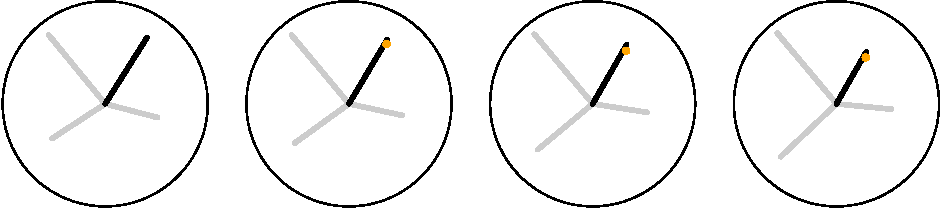
\includegraphics[width=1\linewidth]{paper_files/figure-latex/manualsequence-1} \caption{Sequence of projections where contribution of one variable is controlled (black) is changed using unconstrained orthonormalisation. The dot (orange) indicates the chosen values for the controlled variable. It can be seen that the actual axis does not precisely match the chosen position, but it is close.}\label{fig:manualsequence}
\end{figure}

\hypertarget{refinements-to-enforce-exact-position}{%
\subsection{Refinements to enforce exact
position}\label{refinements-to-enforce-exact-position}}

The problem with new simple method (Algorithm 1) is that the precise
values for \(V_m\) are not followed because the orthonormalisation will
change them. There are numerous ways that this can be enforced, and
details are provided in the Appendix.

\hypertarget{manual-control-for-slice-center}{%
\subsection{Manual control for slice
center}\label{manual-control-for-slice-center}}

How does it work?

Diagram of interface? Scaling

\hypertarget{sec:implementation}{%
\section{Experimenting with new techniques using
Mathematica}\label{sec:implementation}}

\begin{itemize}
\tightlist
\item
  \textbf{Why is this a good sandbox}
\item
  \textbf{Explain the functionality available in the notebooks}
\end{itemize}

\begin{figure}

{\centering 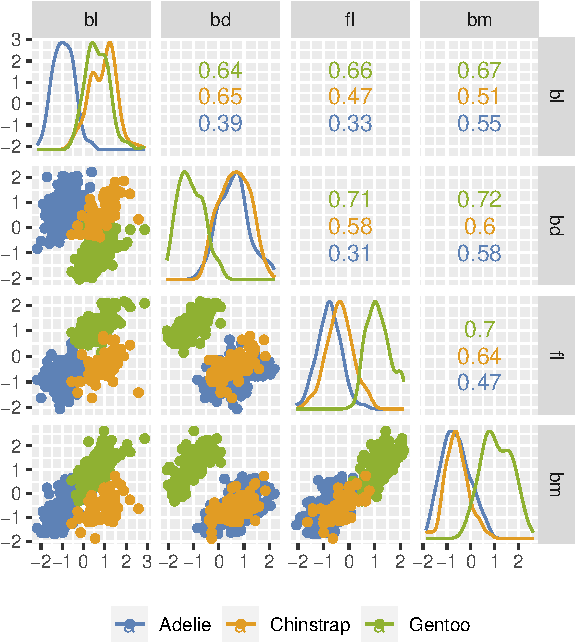
\includegraphics[width=0.8\linewidth]{paper_files/figure-latex/penguins-scatmat-1} 

}

\caption{Scatterplot matrix of the (standardised) penguins data. The three species are reasonably different in size, with Gentoo distinguised from the other two on body depth relative to flipper length and body mass.}\label{fig:penguins-scatmat}
\end{figure}

\hypertarget{sec:examples}{%
\section{Application}\label{sec:examples}}

To illustrate the usefulness of the manual controls we use the 4D
penguins data \citep{penguins}. We will show how classification
boundaries can be explored and better understood on projections and
slices through 4D space. Figure \ref{fig:penguins-scatmat} shows a
scatterplot matrix of this data. There are four variables
(\texttt{bl\ =\ bill\_length\_mm,\ bd\ =\ bill\_depth\_mm,\ fl\ =\ flipper\_length\_mm,\ bm\ =\ body\_mass\_g})
measuring the size of the penguins from three species (Adelie, Chinstrap
and Gentoo). The scatterplot matrix shows that the three species appear
to be likely separable, and that at least the Gentoo can be
distinguished from the other two species when \texttt{bd} is paired with
\texttt{fl} or \texttt{bm}. The steps for exploring boundaries in this
example are as follows:

\begin{enumerate}
\def\labelenumi{\arabic{enumi}.}
\tightlist
\item
  Build your classification model.
\item
  Predict the class for a dense grid of values covering the data space.
\item
  Examine projections, using a manual tour so that the contribution of
  any variable is controlled.
\item
  Slice through the center, to explore where the boundaries will likely
  meet.
\item
  Move the slice by changing the center in the direction of a single
  variable to explore the extent of a boundary for a single group
  relative to a variable.
\end{enumerate}

\hypertarget{constructing-the-4d-prediction-regions}{%
\subsection{Constructing the 4D prediction
regions}\label{constructing-the-4d-prediction-regions}}

We use the \texttt{classifly} package \citep{classifly} to generate
predictions across the 4D cube spanned by the data, with two
classification models: linear discriminant analysis (LDA) and random
forest (RF).

\hypertarget{exploring-projections-manually}{%
\subsection{Exploring projections
manually}\label{exploring-projections-manually}}

We start by first exploring the projections of the model prediction.
Figure \ref{proj1} summarises the process. Through manual rotation of
the view we can get a feeling for where in the space we primarily
predict each of the three species, and we also get a sense of the
difference between the two models. To illustrate this difference we have
manually rotated the projection for the RF model (left plot) to identify
a projection that shows the non-linear but block-type structure that is
typical of this type of model. This particular projection (\(A_1\)) is
exported so that the same projection can be used to show the LDA model
(middle plot) and the actual data (right plot). What can be seen is the
linearity of the LDA model, where the boundaries are linear and oblique
to the variable axes. And, interestingly this particular projection of
the original data shows very distinct clusters of the three species.
That means, the obscuring of the boundaries between groups for both of
the models is driven by what is happening in the orthogonal space to the
plane of the selected projection.

\begin{figure*}[ht]
\centerline{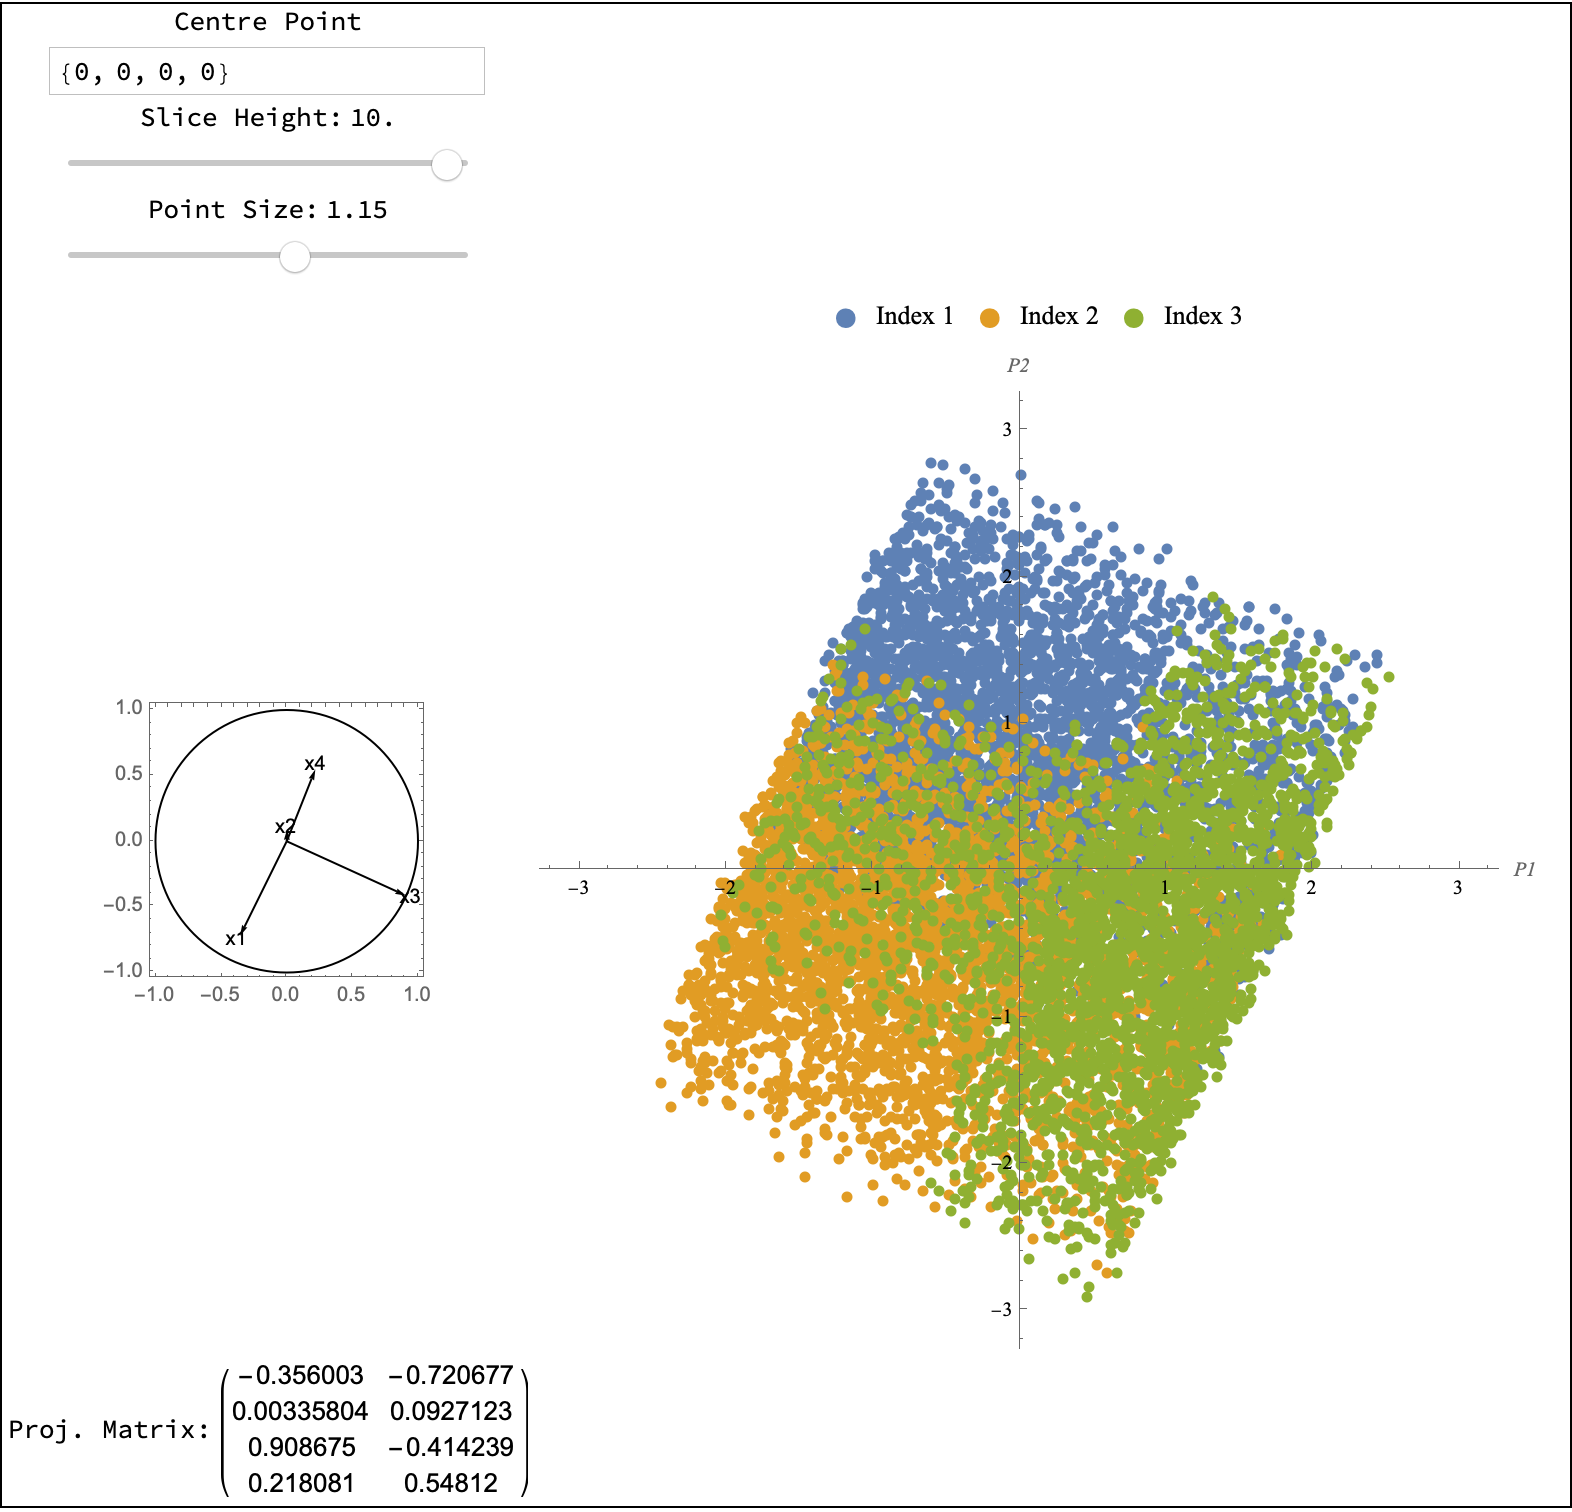
\includegraphics[width=0.32\textwidth]{figures/proj1_rf.png}
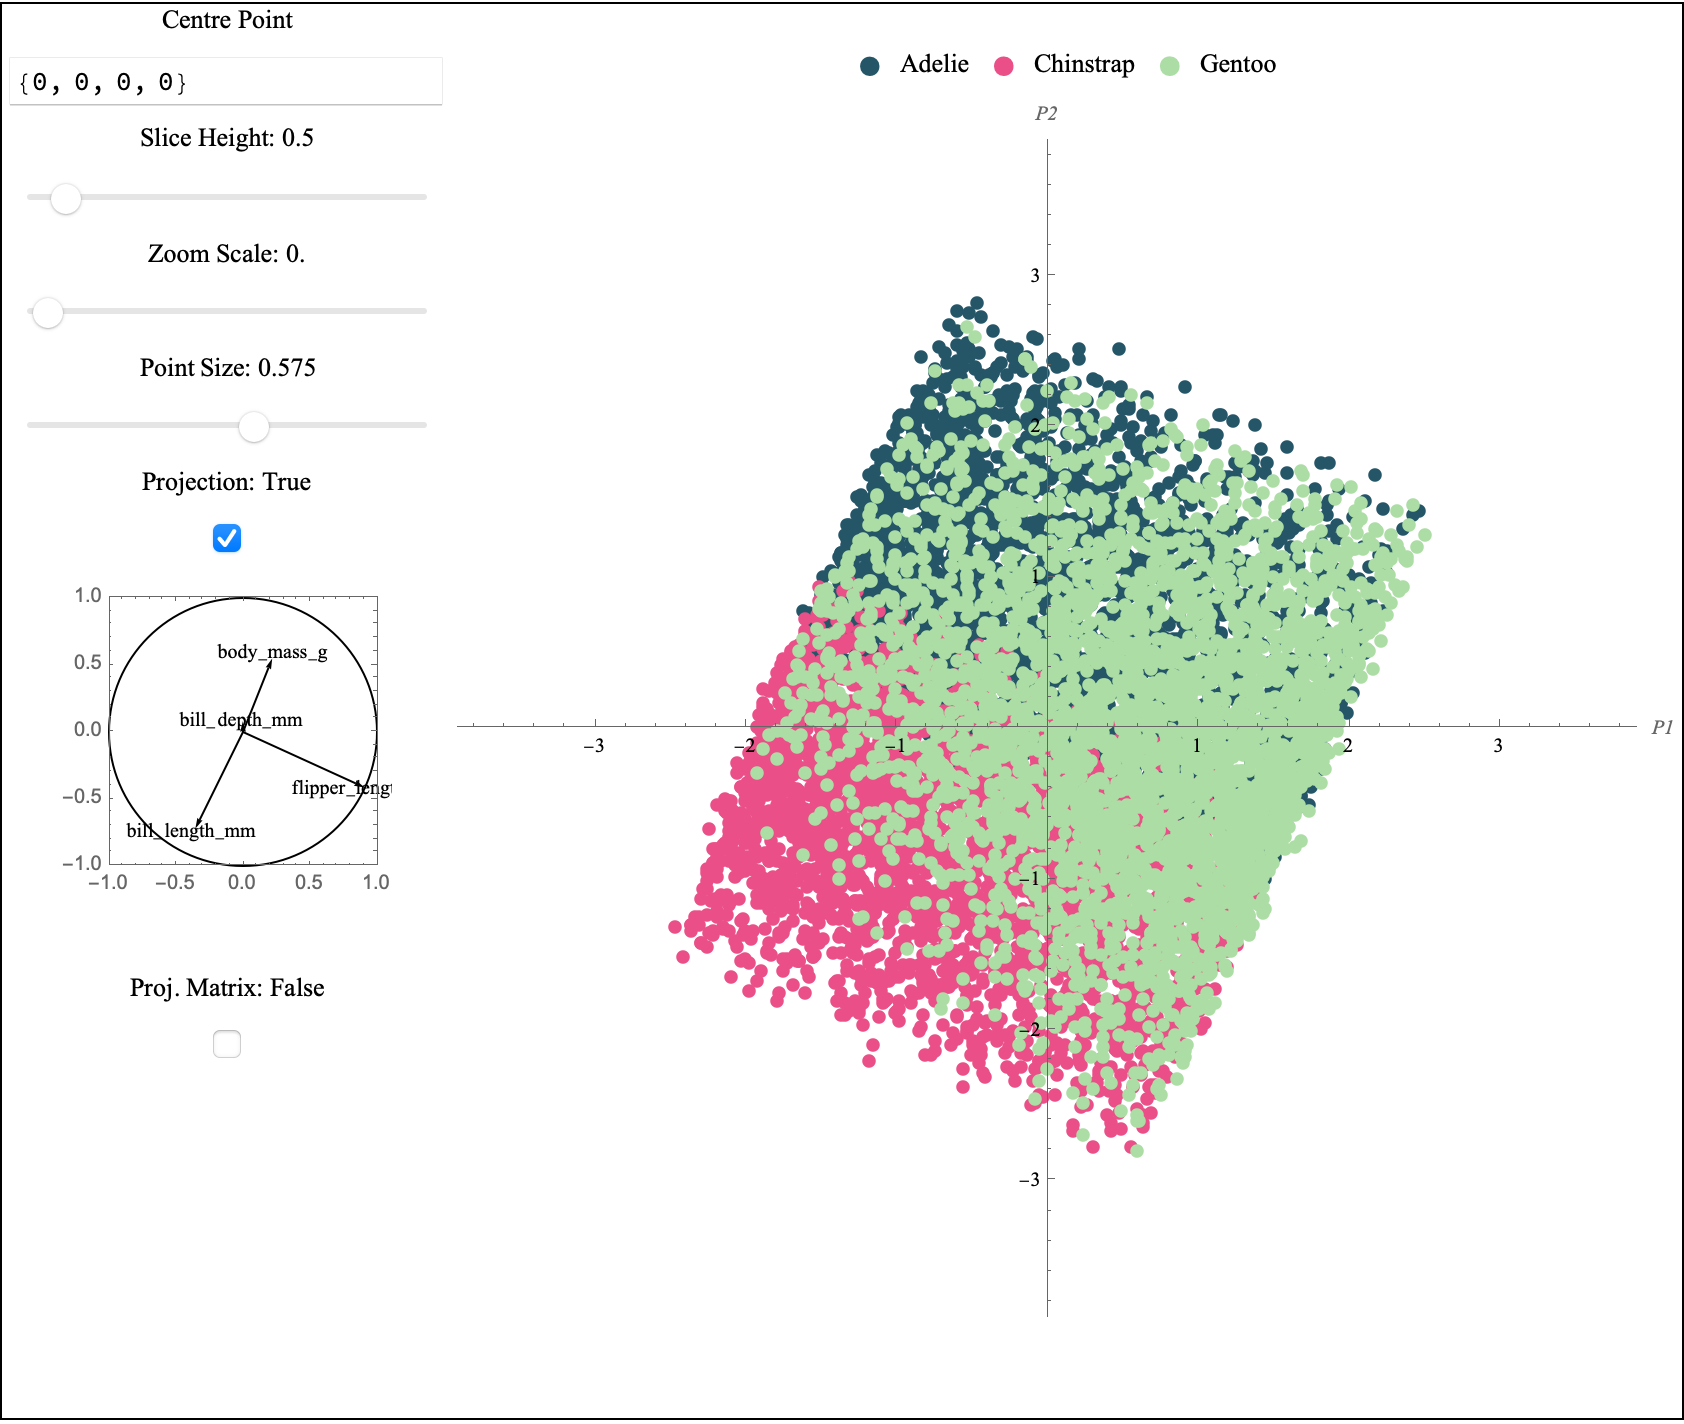
\includegraphics[width=0.32\textwidth]{figures/proj1_lda.png}
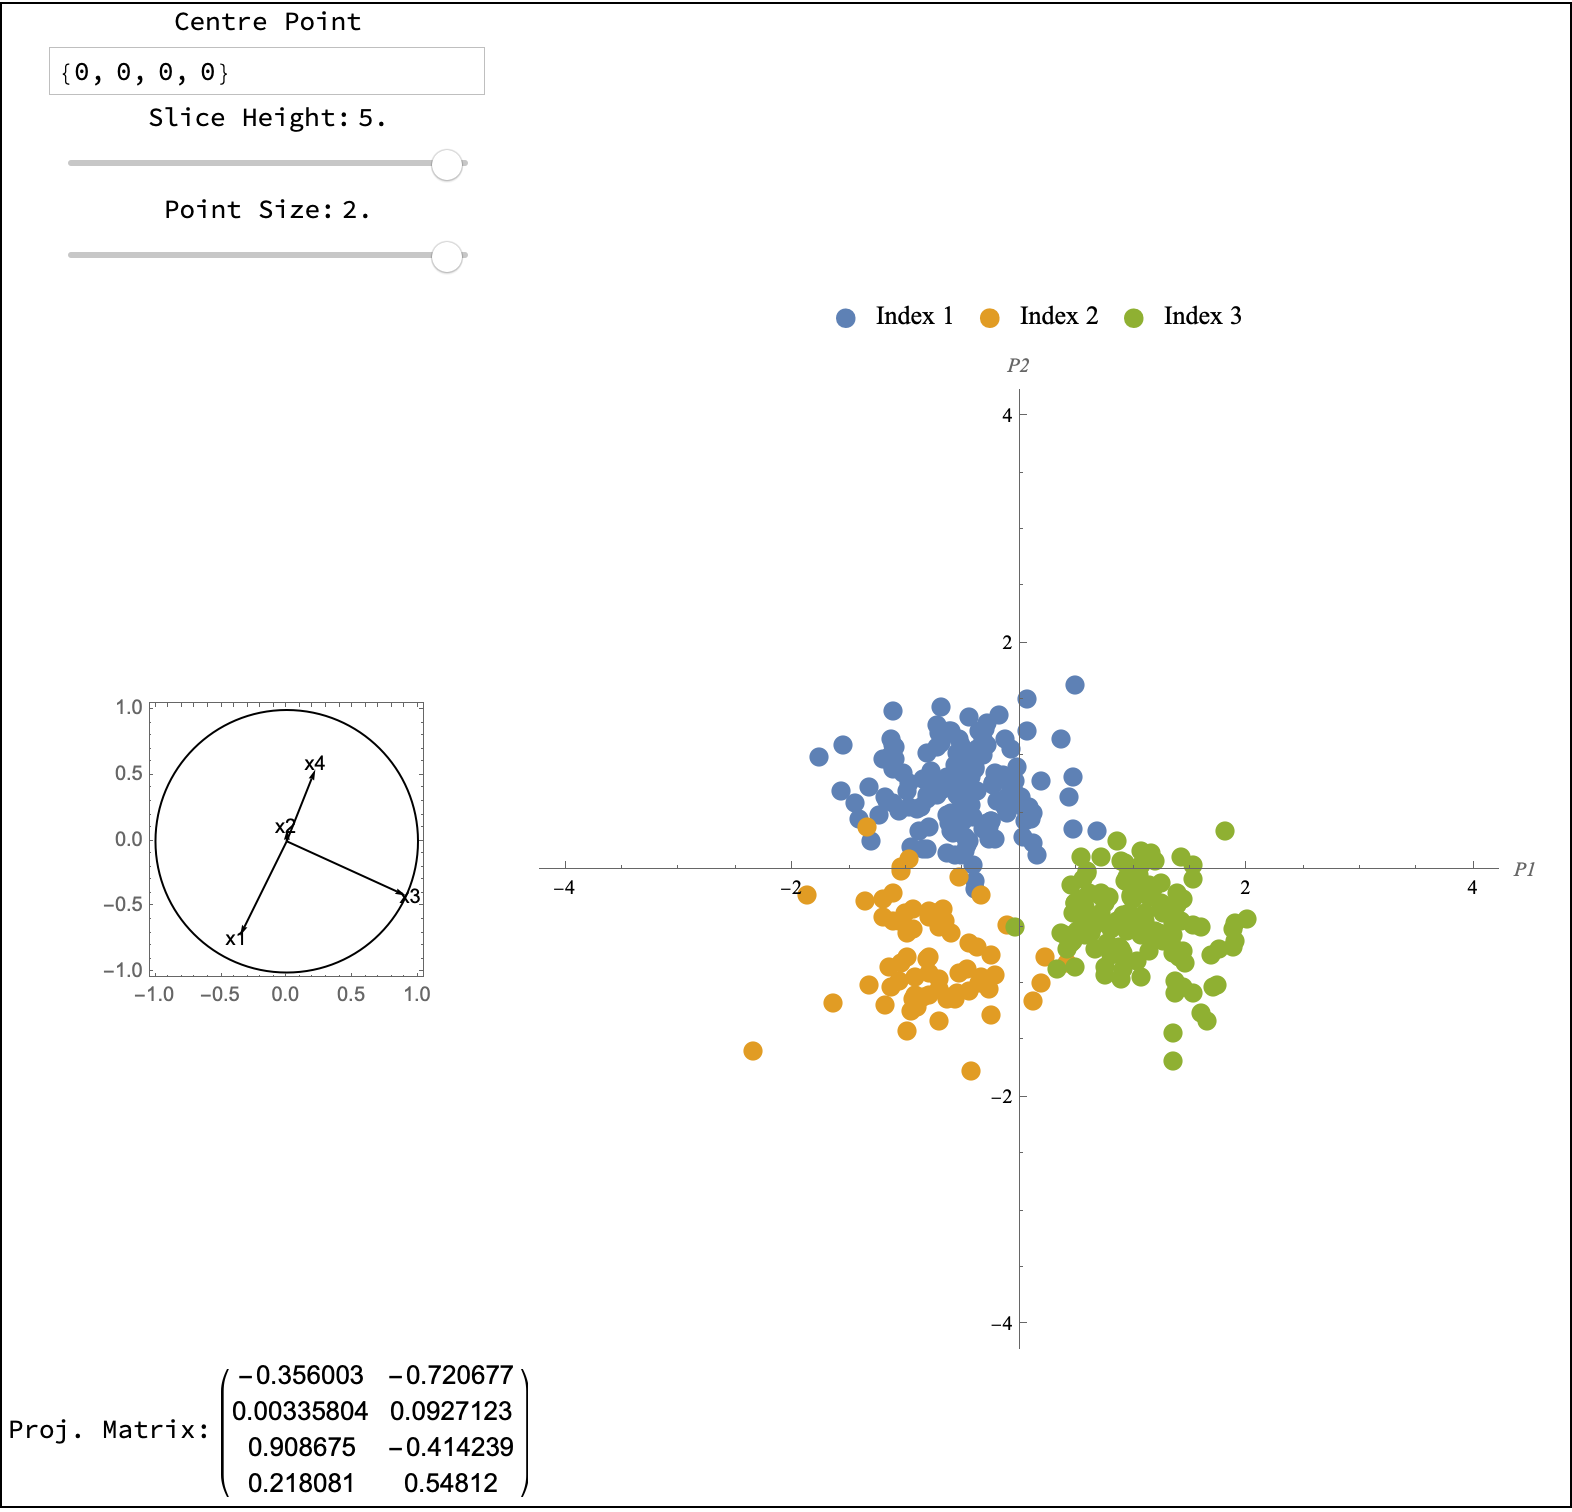
\includegraphics[width=0.32\textwidth]{figures/proj1_data.png}}
\caption{Projection identified using the manual tour, because it reveals an interesting structure in the predictions from the RF model (left). We can clearly see a block structure, while the LDA model (middle) produces linear boundaries. The three groups are nicely separated in this projection of the data (right)}.
\label{proj1}
\end{figure*}

\hypertarget{slicing-through-the-center}{%
\subsection{Slicing through the
center}\label{slicing-through-the-center}}

XXXX currently in the notebook \(A_1\) is called A5, and \(A_2\) is
called A6

We continue the investigation by now slicing based on the projection
\(A_1\). For both models we look at a thin (\(h=0.5\)) slice through the
center, \(S_1^0\). As a first option we explore how manually changing
the projection away from \(A_1\) can help with understanding the
boundary better. For our example we notice that \(A_1\) does not contain
any contribution from the second variable (\texttt{bd}), and in our
illustration we will first rotate this variable into the view.

We again start by looking at the RF model, the slice \(S_1^0\) shows the
block structure of the model, with the third group (green, Gentoo
penguins) overlapping with both of the other groups (Fig. \ref{slice1},
top-left). This is similar for the LDA model (Fig. \ref{slice1},
top-right), but again the linearity results in different boundaries and
thus differences in how the classes overlap.

By rotating in the second variable we can find a view that shows three
neatly separated blocks for the RF model, and we export the
corresponding projection matrix \(A_2\) to see the same views for the
LDA model which also shows a neater separation of the classes along the
boundary (see bottom row of Fig. \ref{slice1}).

Finally we look at the data projection based on \(A_2\) and find that
the third group (green, Gentoo penguins) is further away from the other
two groups (compared to \(A_1\)), see Fig. \ref{proj2}.

\begin{figure*}[ht]
\centerline{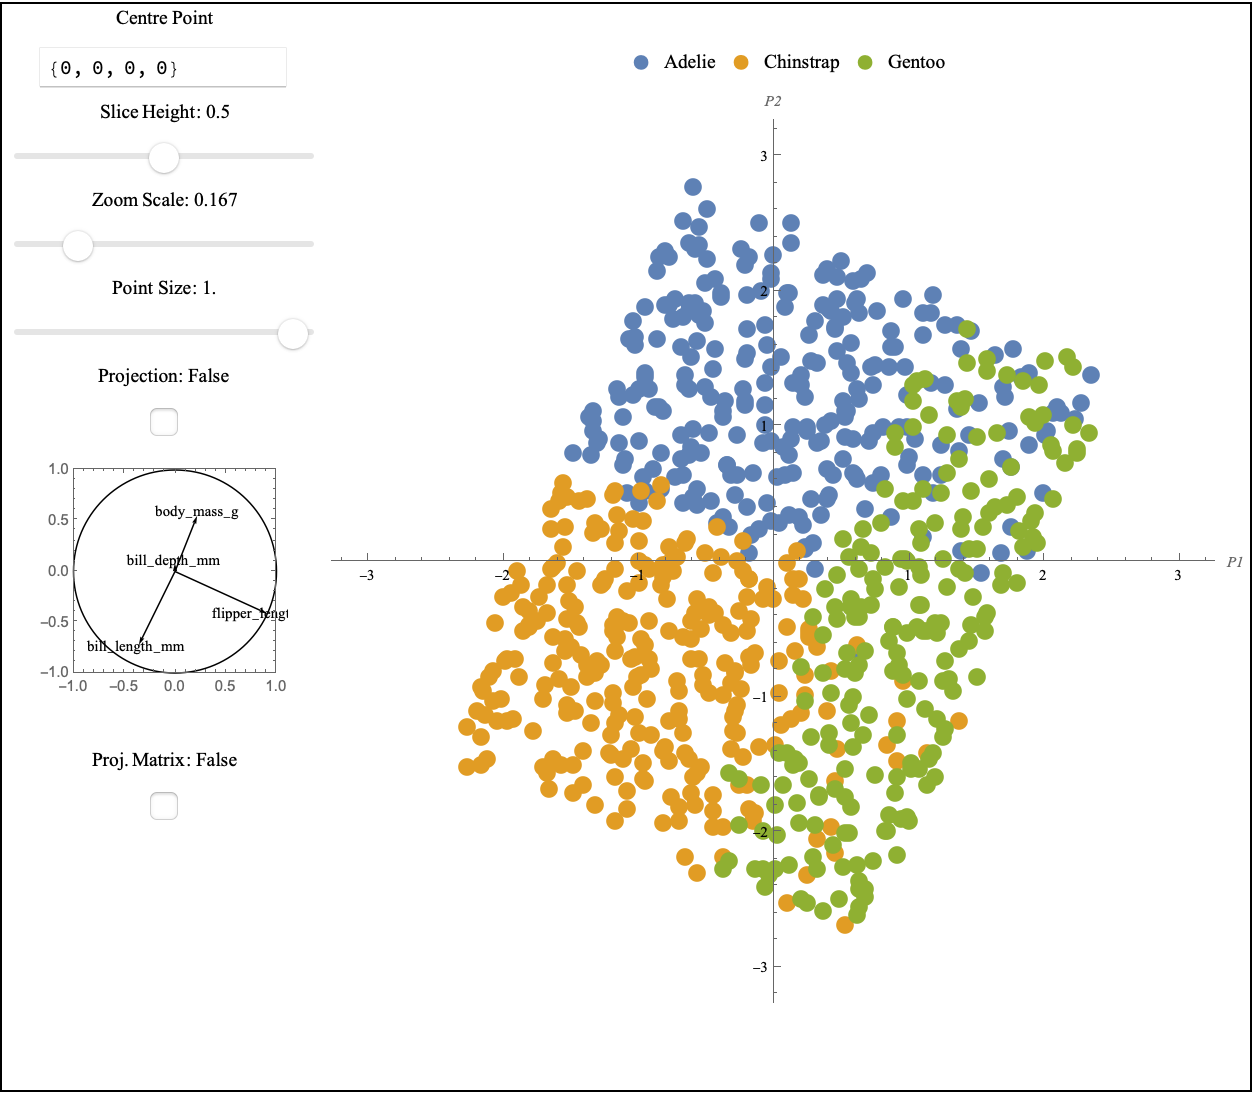
\includegraphics[width=0.45\textwidth]{figures/slice1_rf.png}
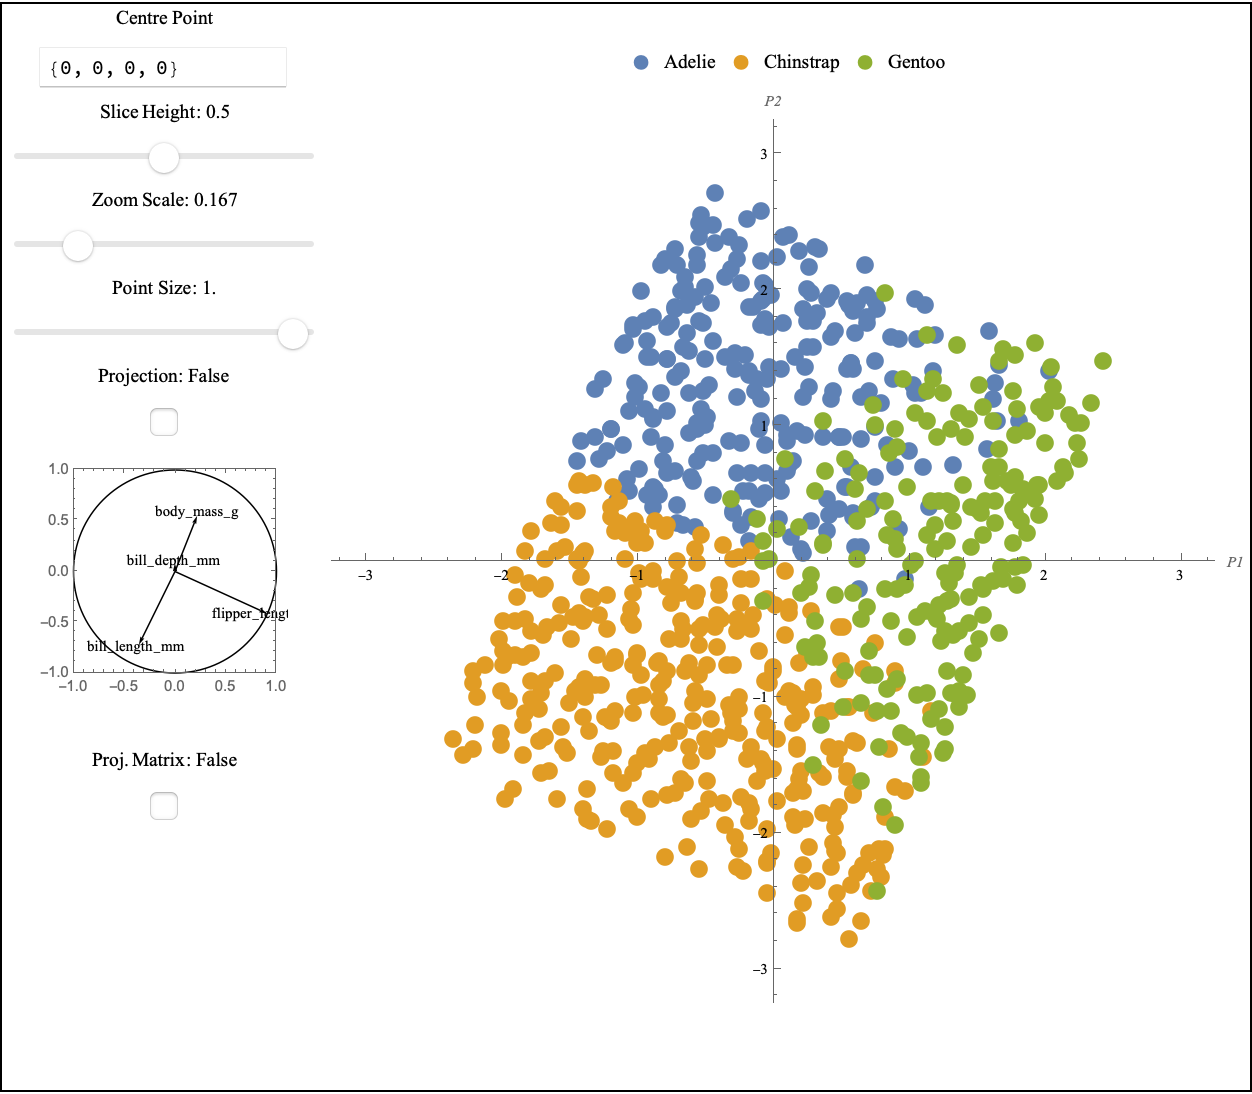
\includegraphics[width=0.45\textwidth]{figures/slice1_lda.png}}
\centerline{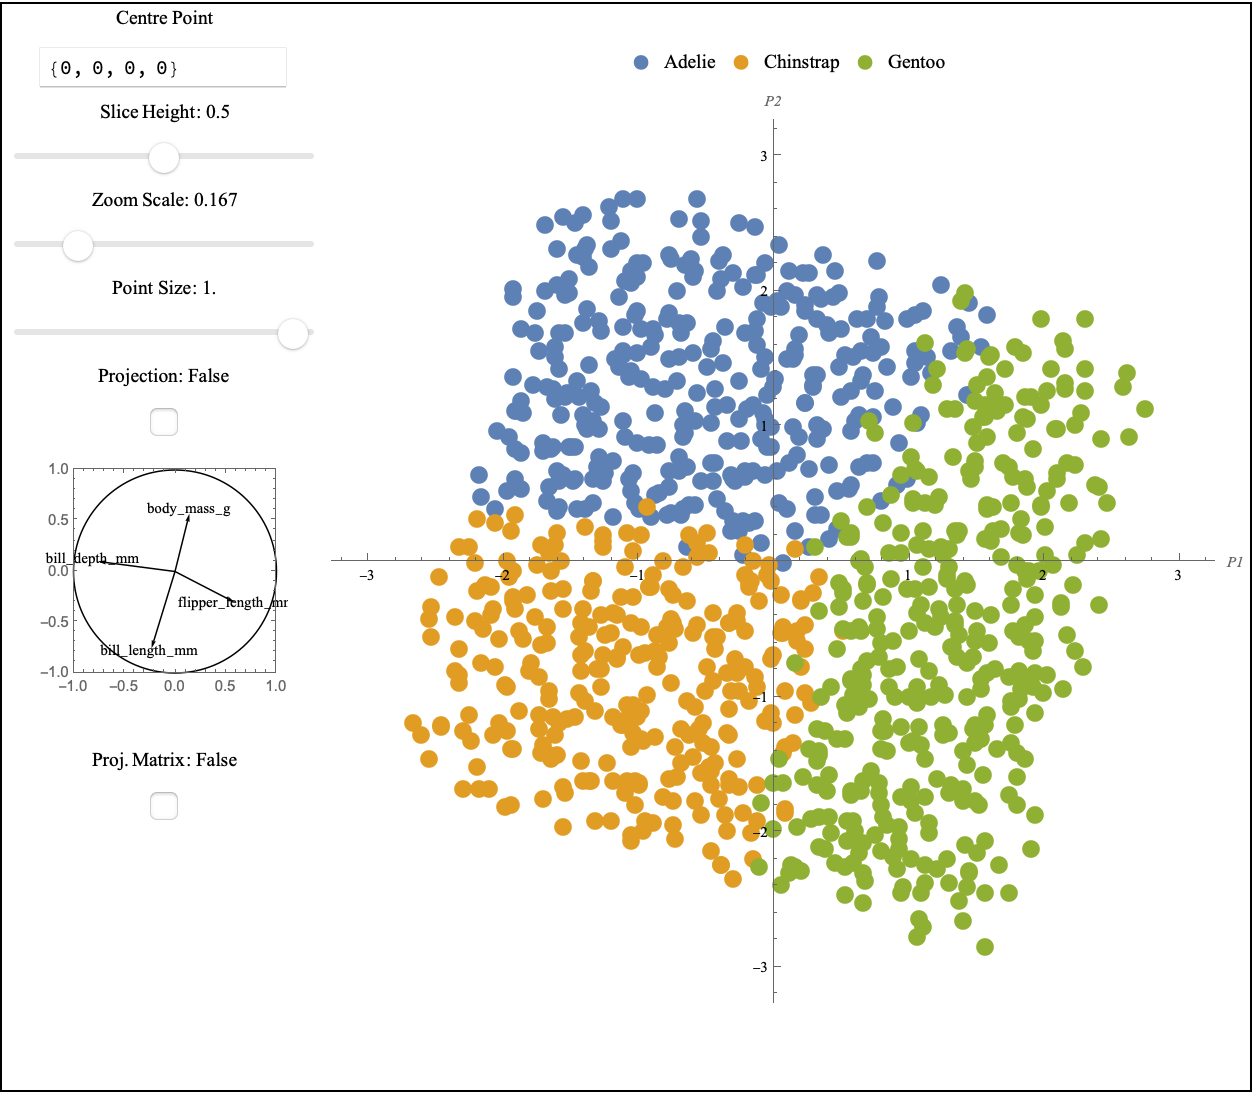
\includegraphics[width=0.45\textwidth]{figures/slice2_rf.png}
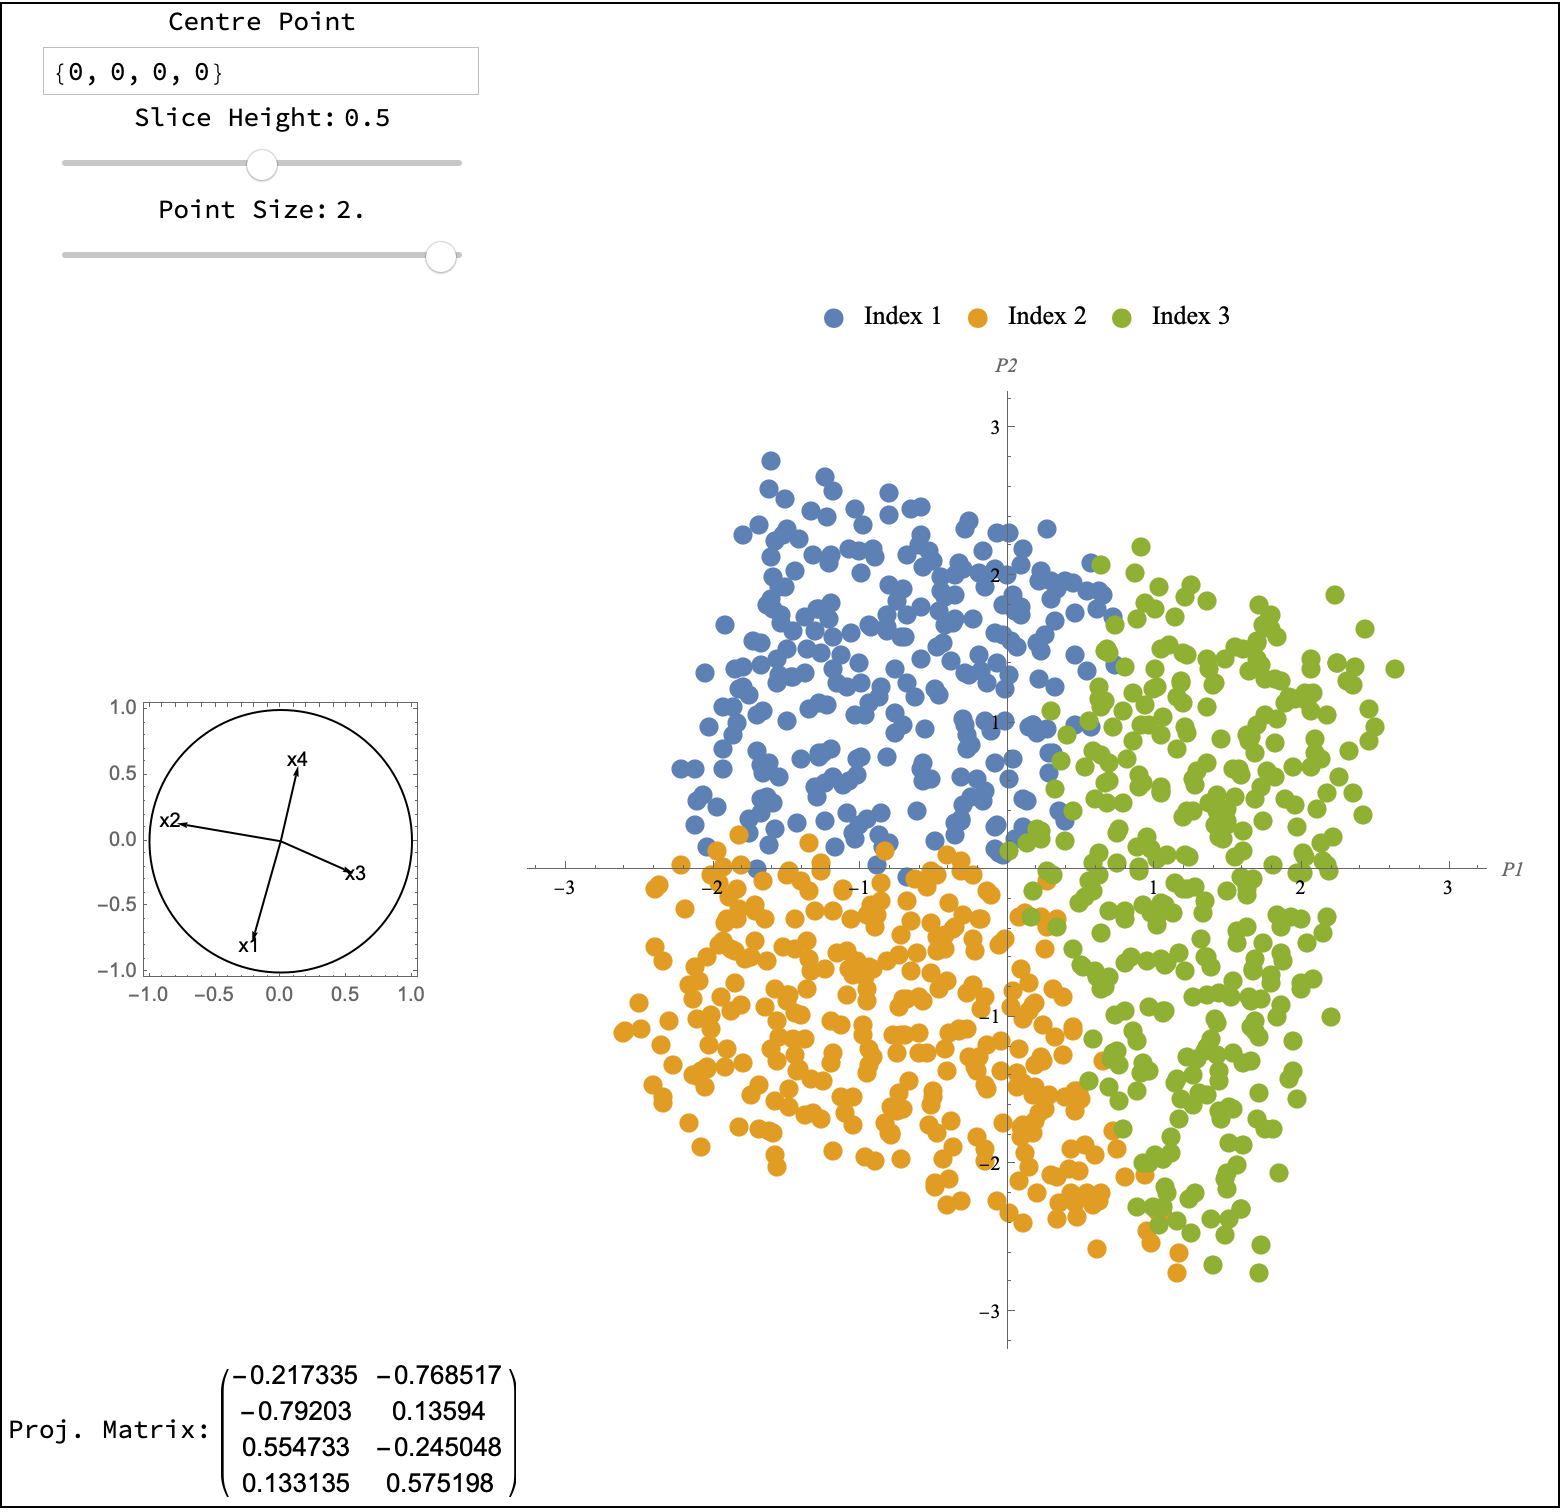
\includegraphics[width=0.45\textwidth]{figures/slice2_lda.png}}
\caption{Comparing slices based on two projections $A_1$ (top row) and $A_2$ (bottom row), for the two models RF (left) and LDA (right). With $A_1$ we see two groups overlap (green - Gentoo with yellow - Chinstrap), while the rotation to $A_2$ results in clear boundaries inside the slice. The boundary between Adelie (blue) and Chinstrap (yellow) is similar for both models but very different between Chinstrap and Gentoo (green).}
\label{slice1}
\end{figure*}

\begin{figure*}[ht]
\centerline{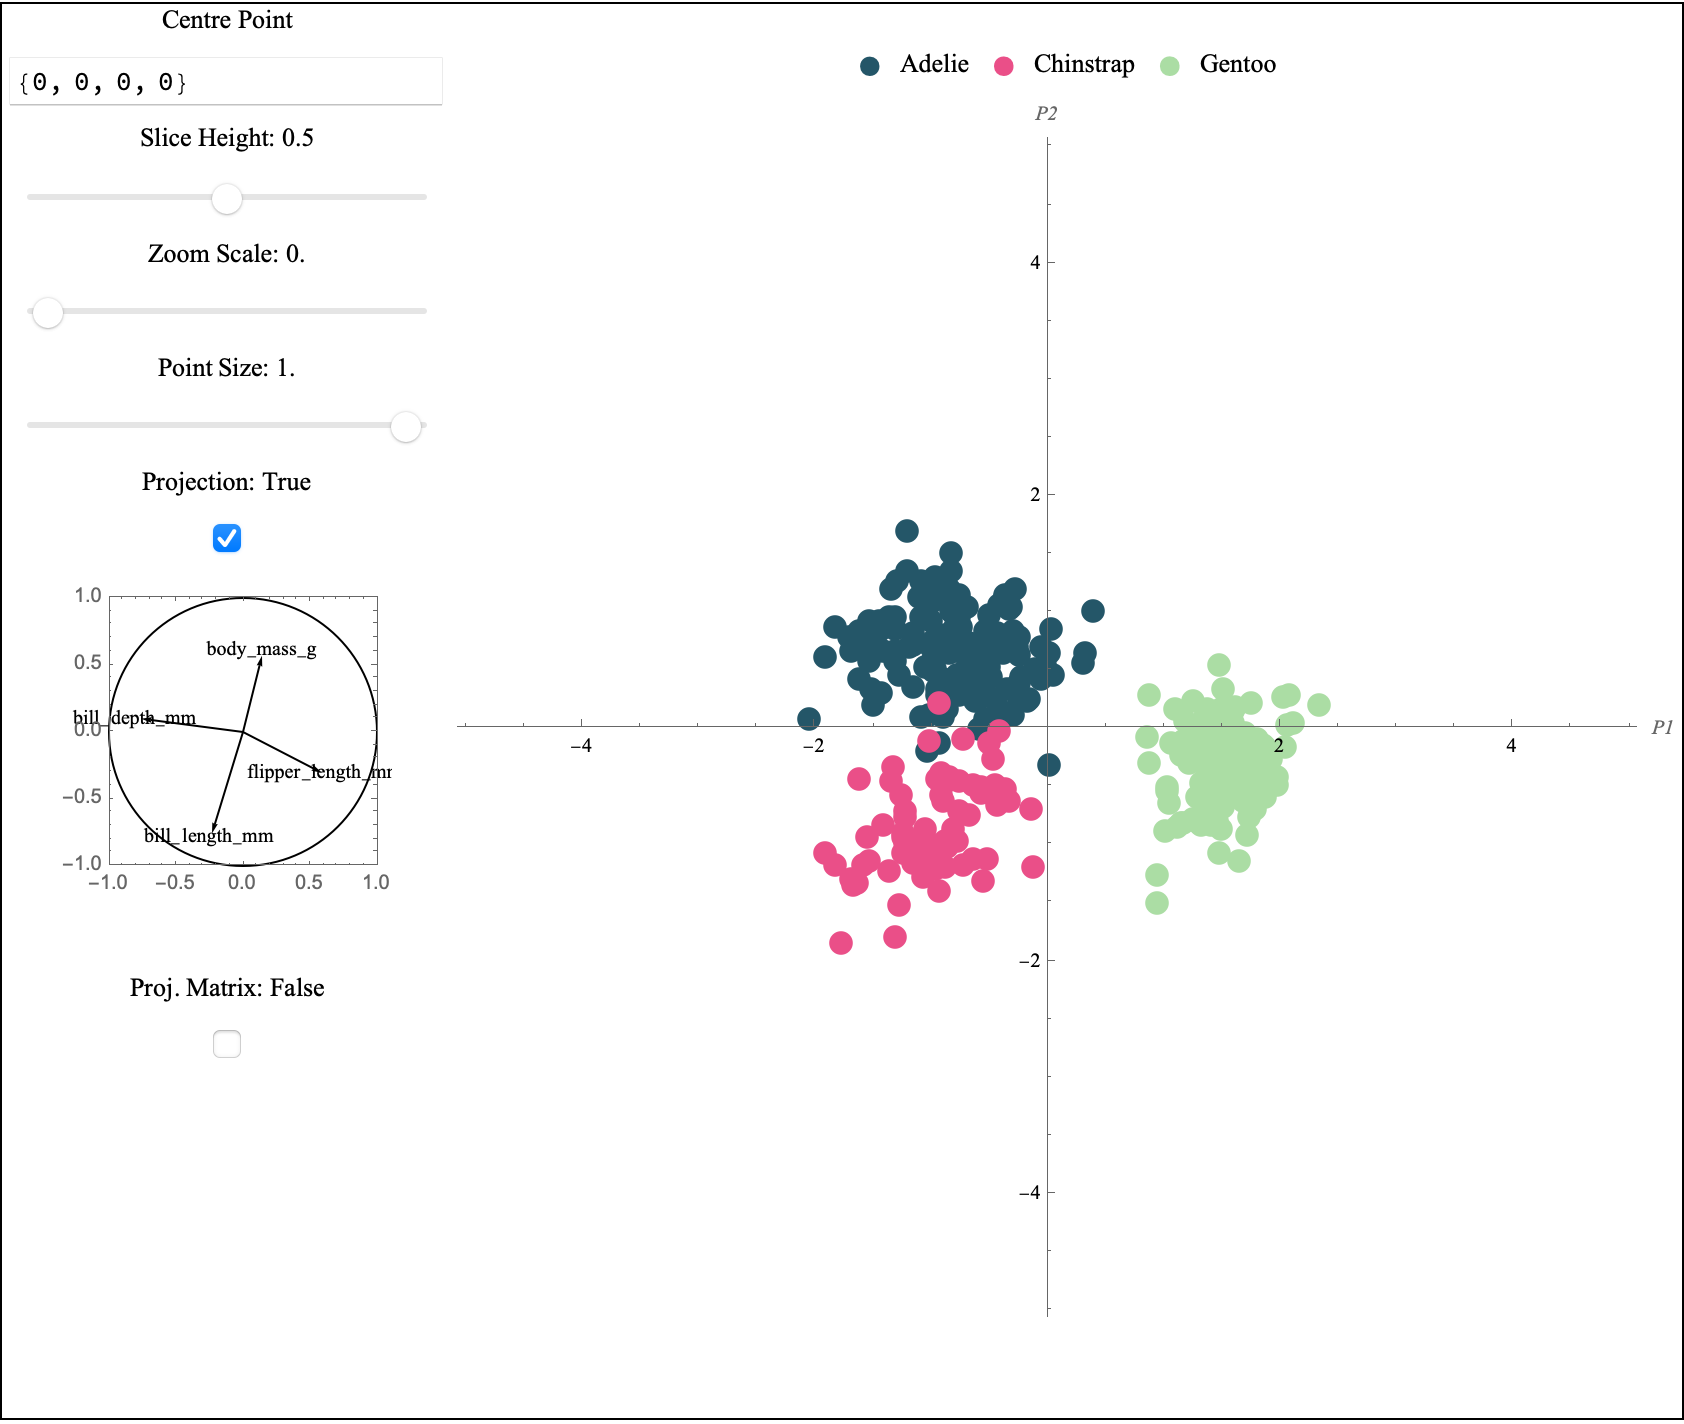
\includegraphics[width=0.45\textwidth]{figures/proj2_data.png}}
\caption{Projection of the data based on $A_2$. Compared to projecting onto $A_1$ we see that the green observations (Gentoo) are more separated from the other two species.}
\label{proj2}
\end{figure*}

\hypertarget{shifting-the-slice-center}{%
\subsection{Shifting the slice center}\label{shifting-the-slice-center}}

We have seen that starting from \(A_1\) using the manual controls to
change the contribution of the second variable we could find a clear
separation boundary indicating the relation between this variable (bill
depth) and the Gentoo penguin species. Instead of rotating to a
different projection, we might also change the view by moving the slice
along one direction in the 4D space. Here we will continue our
exploration of the dependence on \texttt{bd} and move the slice defined
by \(A_1\) to either large or small values of the bill depth
(\(\pm 1.5\) after centering and scaling). We will label these slices as
\(S_1^{\pm}\). Here we will also look at slices of the observed data
points, using a thicker slice (\(h=1.5\)) to capture enough points in a
given view.

We start by a comparison of the two models and the data distribution in
\(S_1^{+}\), thus the slice is localized towards high values of bill
depth in Fig. \ref{slice1p}. We can see that all three slices (the two
models and the data) contain almost no points from the third class
(green, Gentoo), and that the decision boundary between the two models
is very similar.

\begin{figure*}[ht]
\centerline{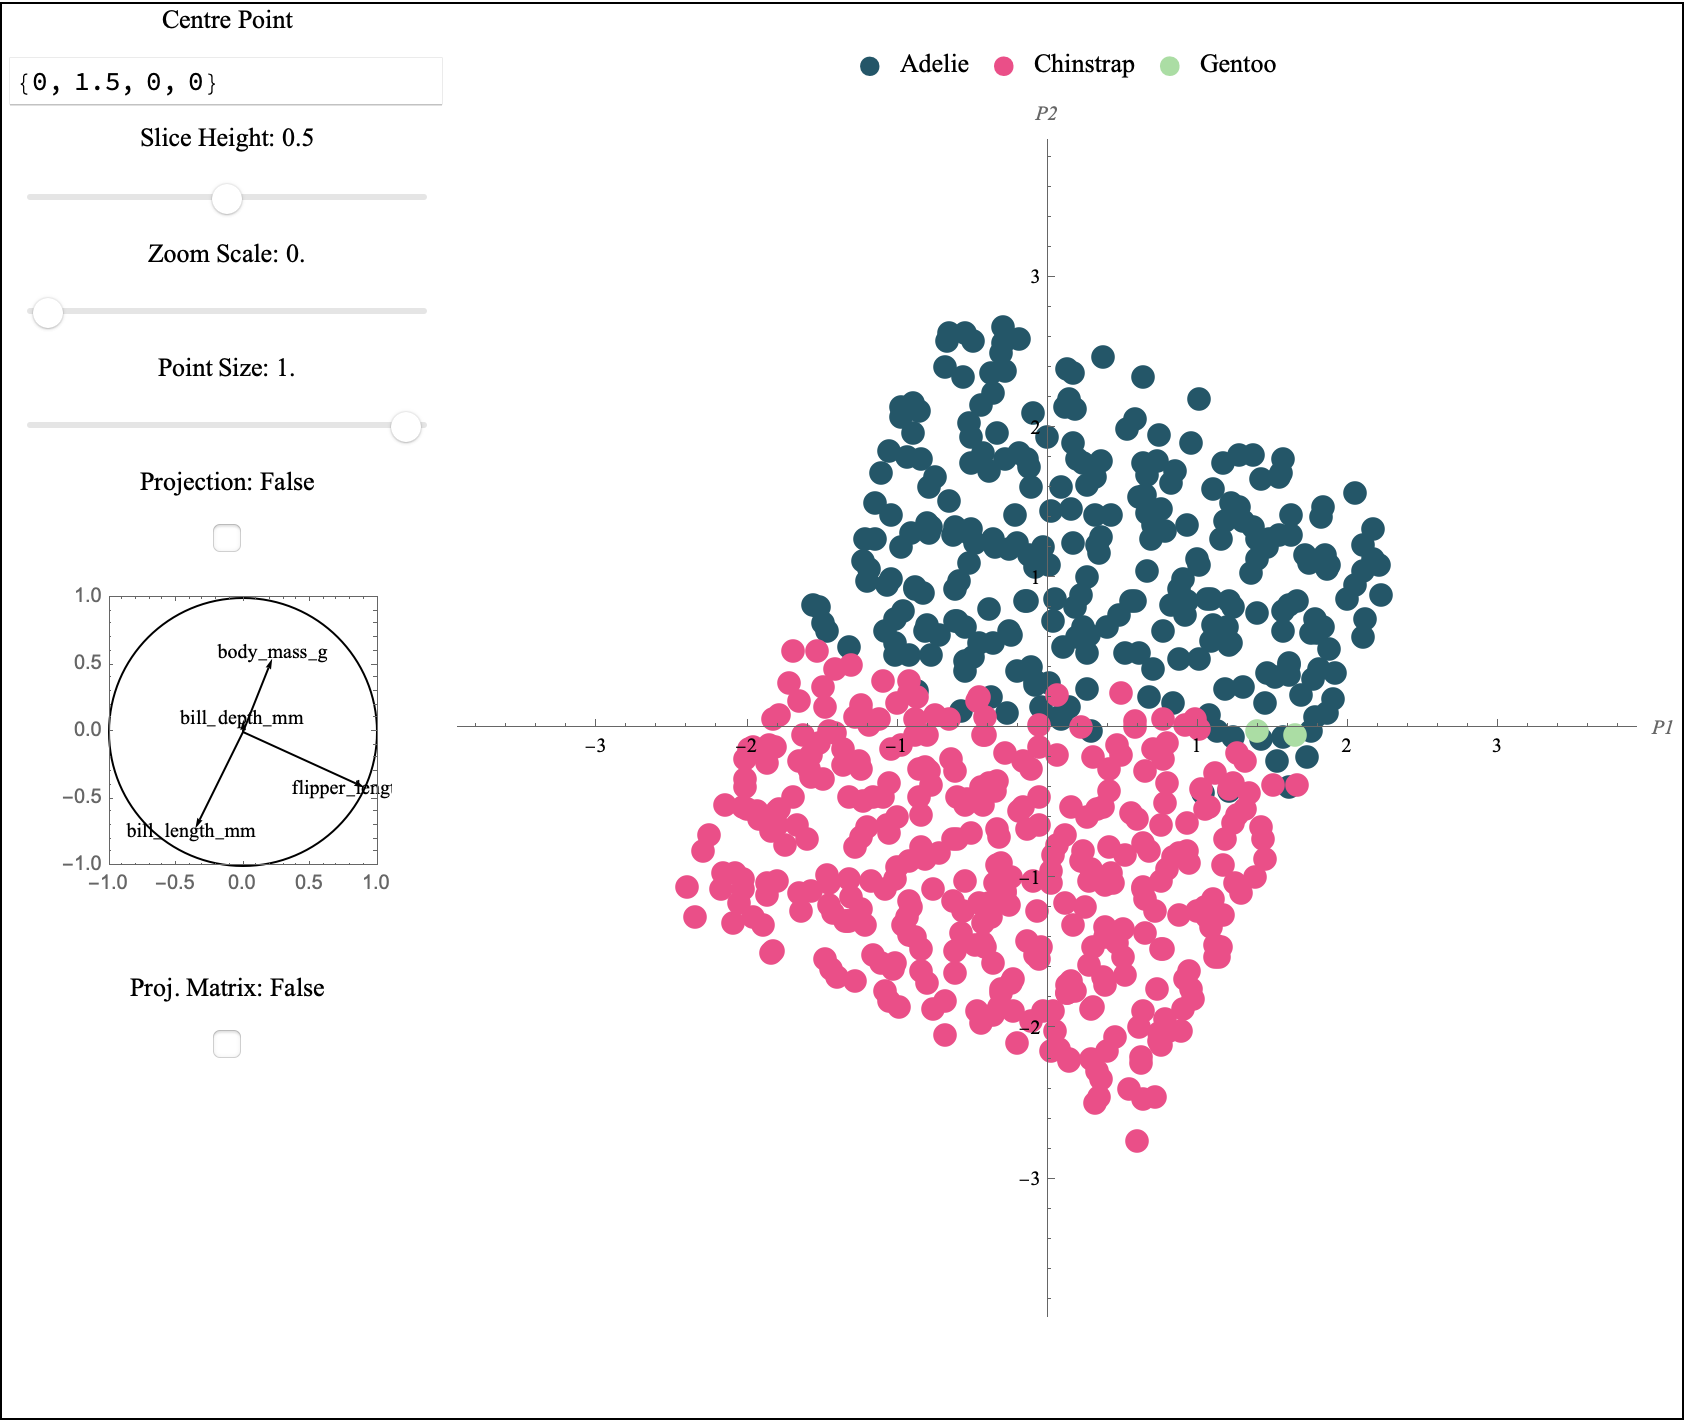
\includegraphics[width=0.32\textwidth]{figures/slice1_p_rf.png}
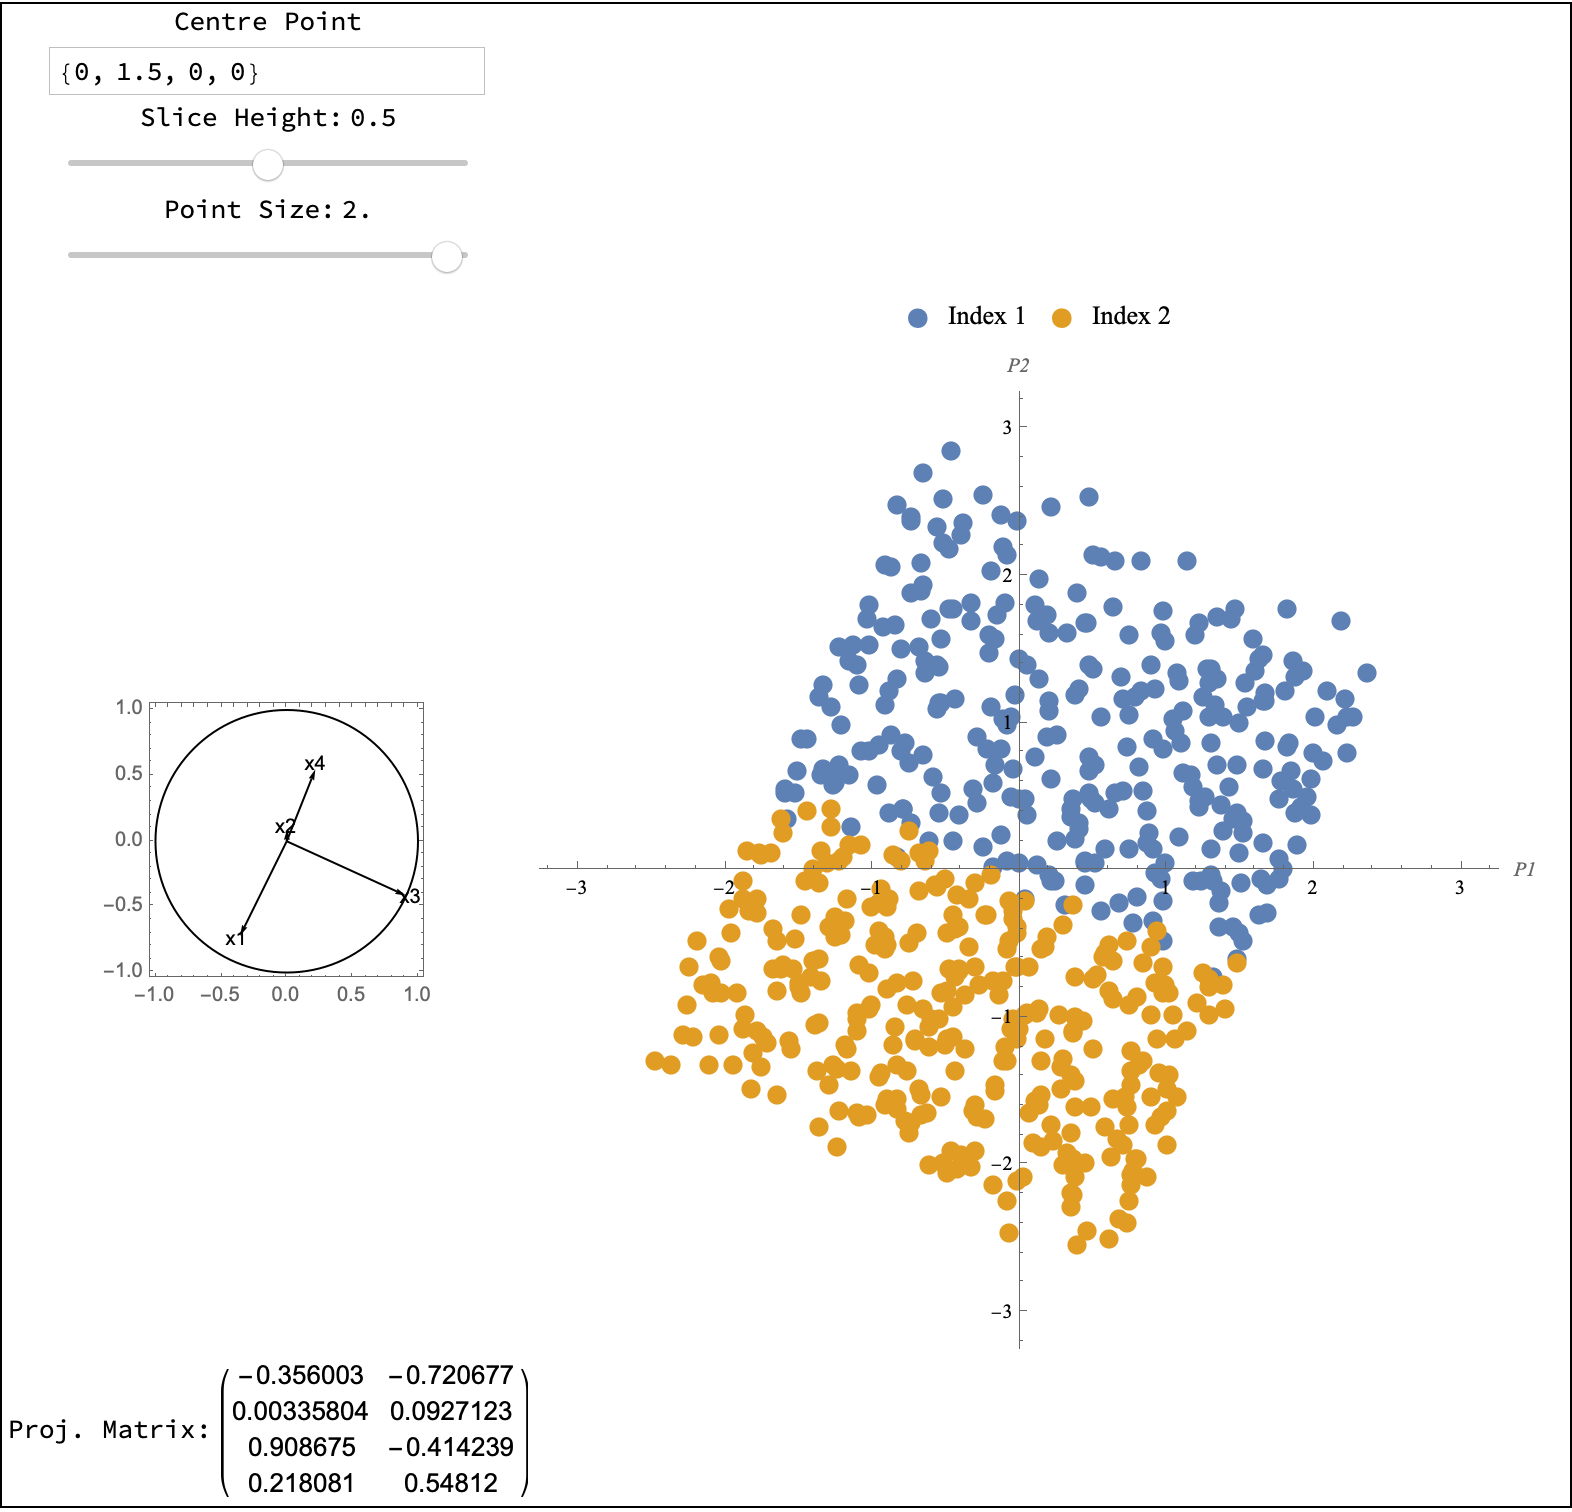
\includegraphics[width=0.32\textwidth]{figures/slice1_p_lda.png}
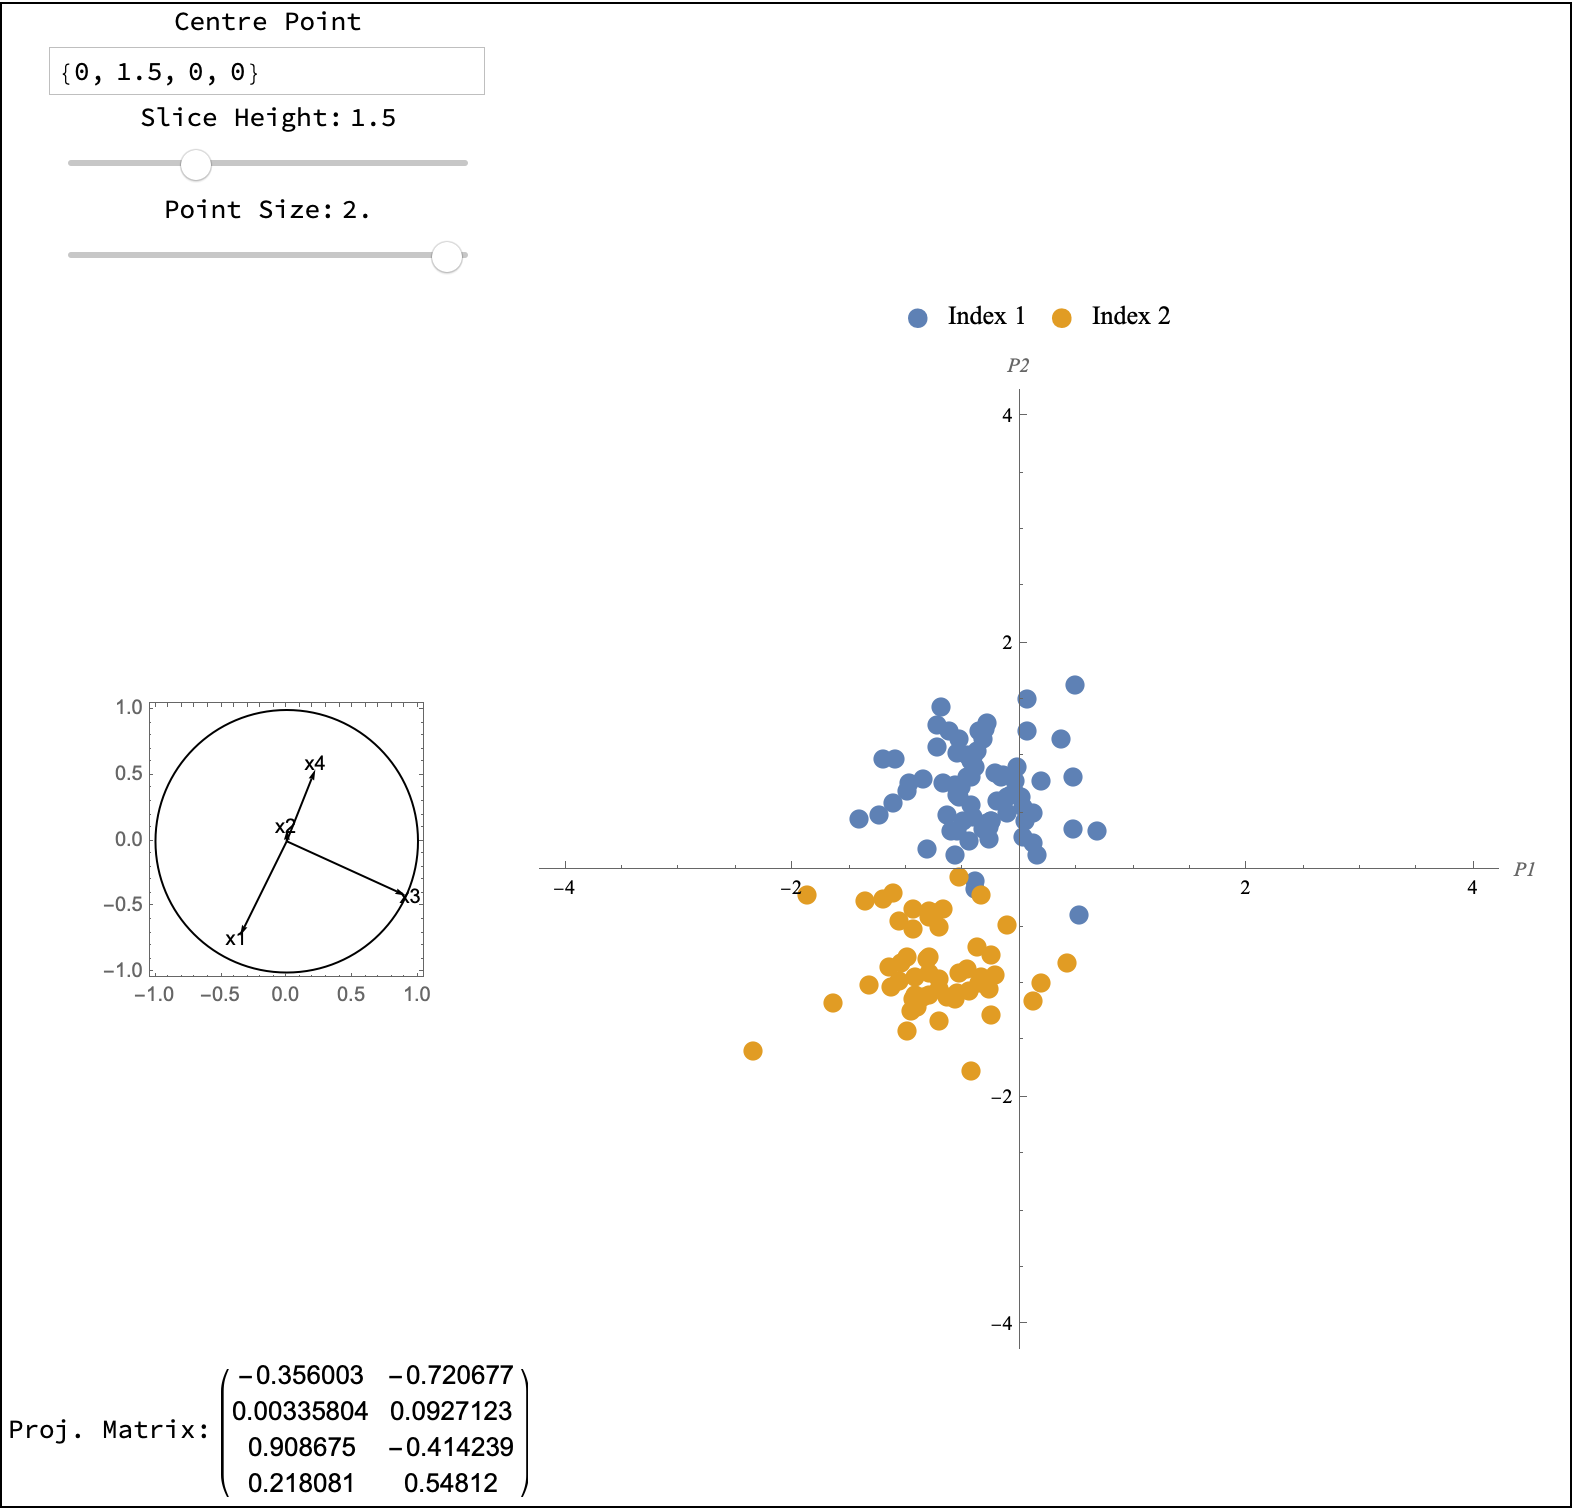
\includegraphics[width=0.32\textwidth]{figures/slice1_p_data.png}}
\caption{...}.
\label{slice1p}
\end{figure*}

A more interesting comparison is found for \(S_1^{-}\), thus the slice
localized towards low values of bill depth, shown in Fig. \ref{slice1m}.
The RF model (left) predicts all three species within this slice, with
an interesting boundary for the third class (green, Gentoo). On the
other hand the LDA model (middle) predominantly predicts the third class
within the slice, this appears to be enforced through the linear
structure of the model. Looking finally at the thick slice through the
data we see that there are primarily observations from this class within
the slice we can conclude that the two models have filled in the
``empty'' space (where we do not have any training observations) in very
different ways and according to what we might expect given the model
structure.

\begin{figure*}[ht]
\centerline{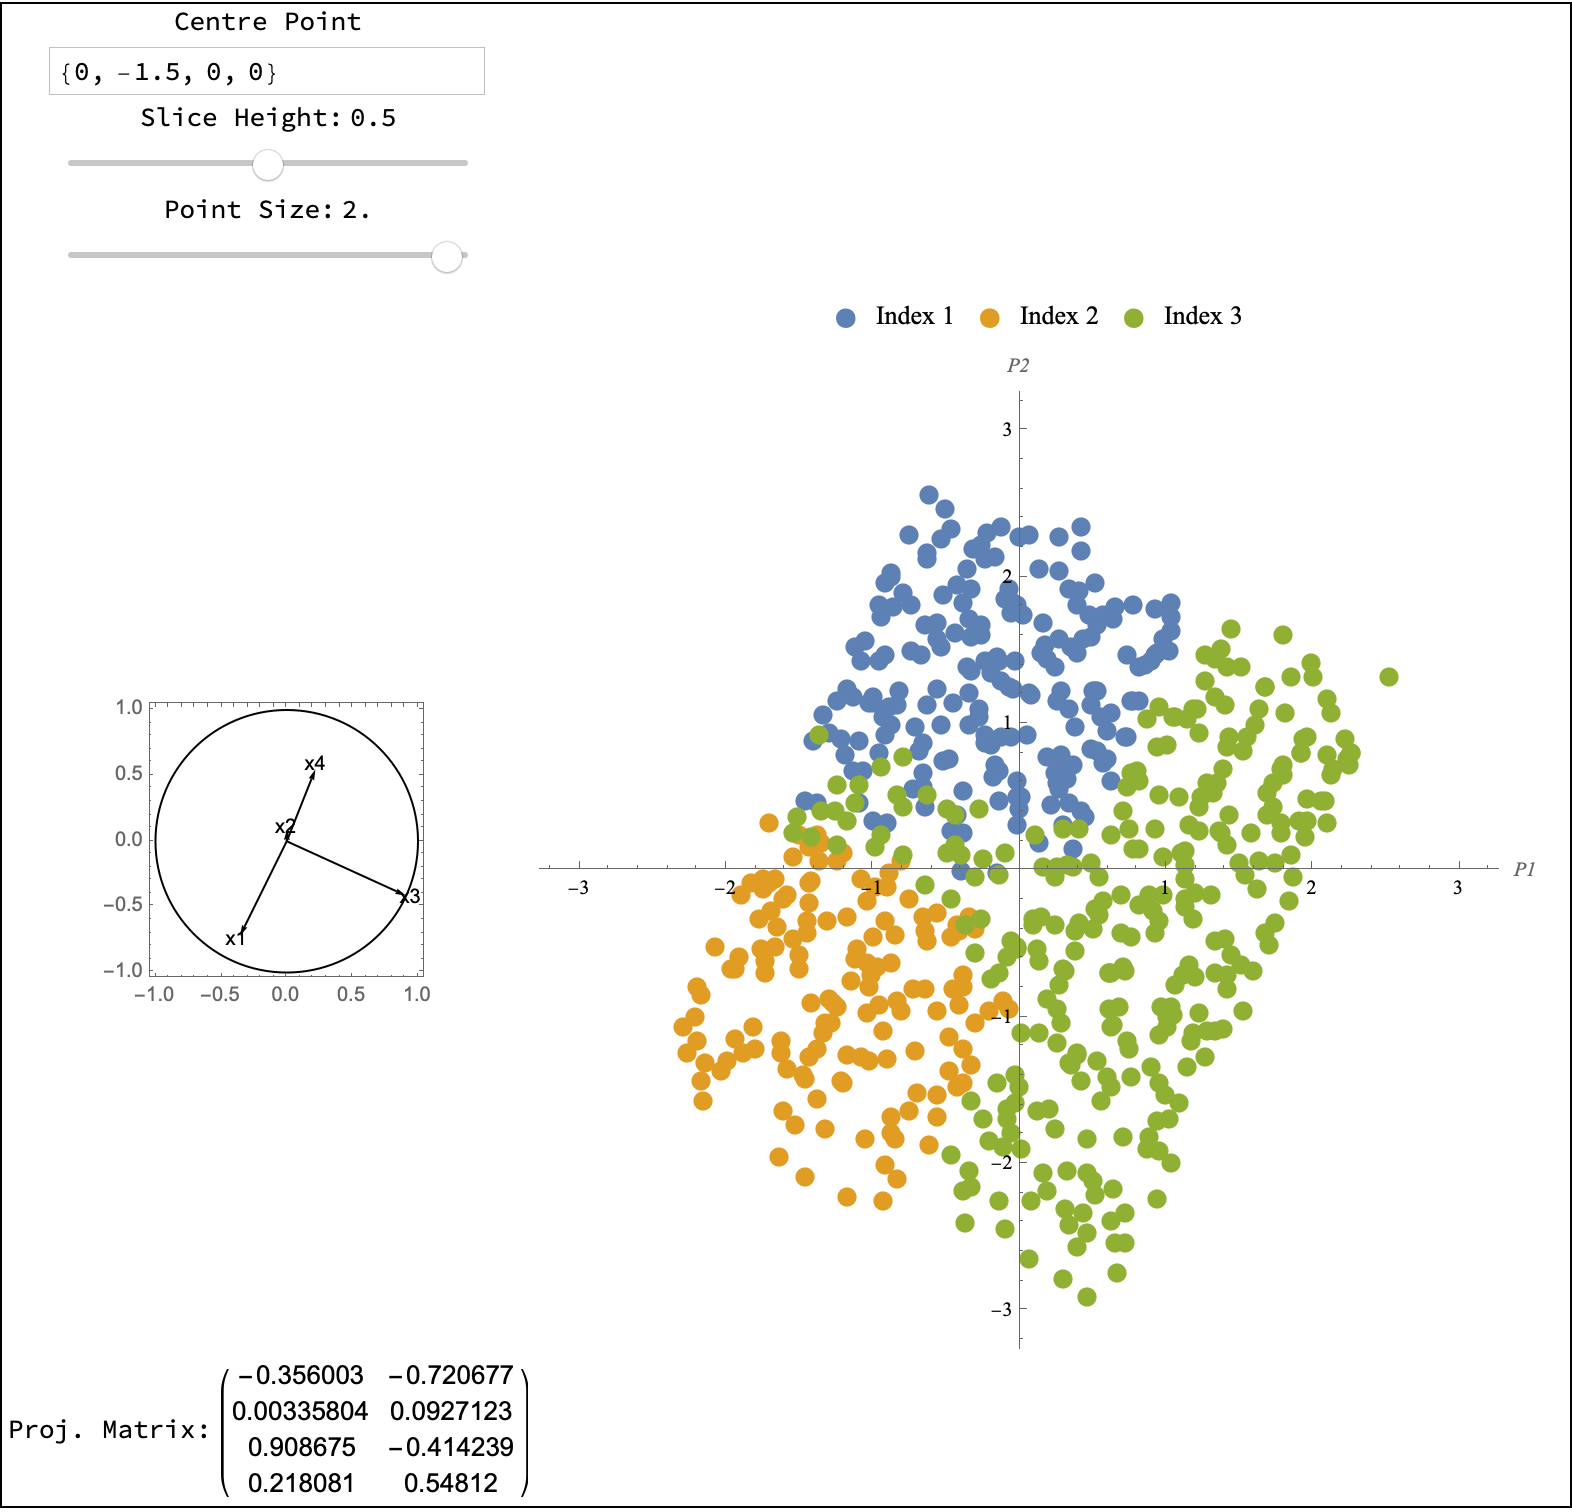
\includegraphics[width=0.32\textwidth]{figures/slice1_m_rf.png}
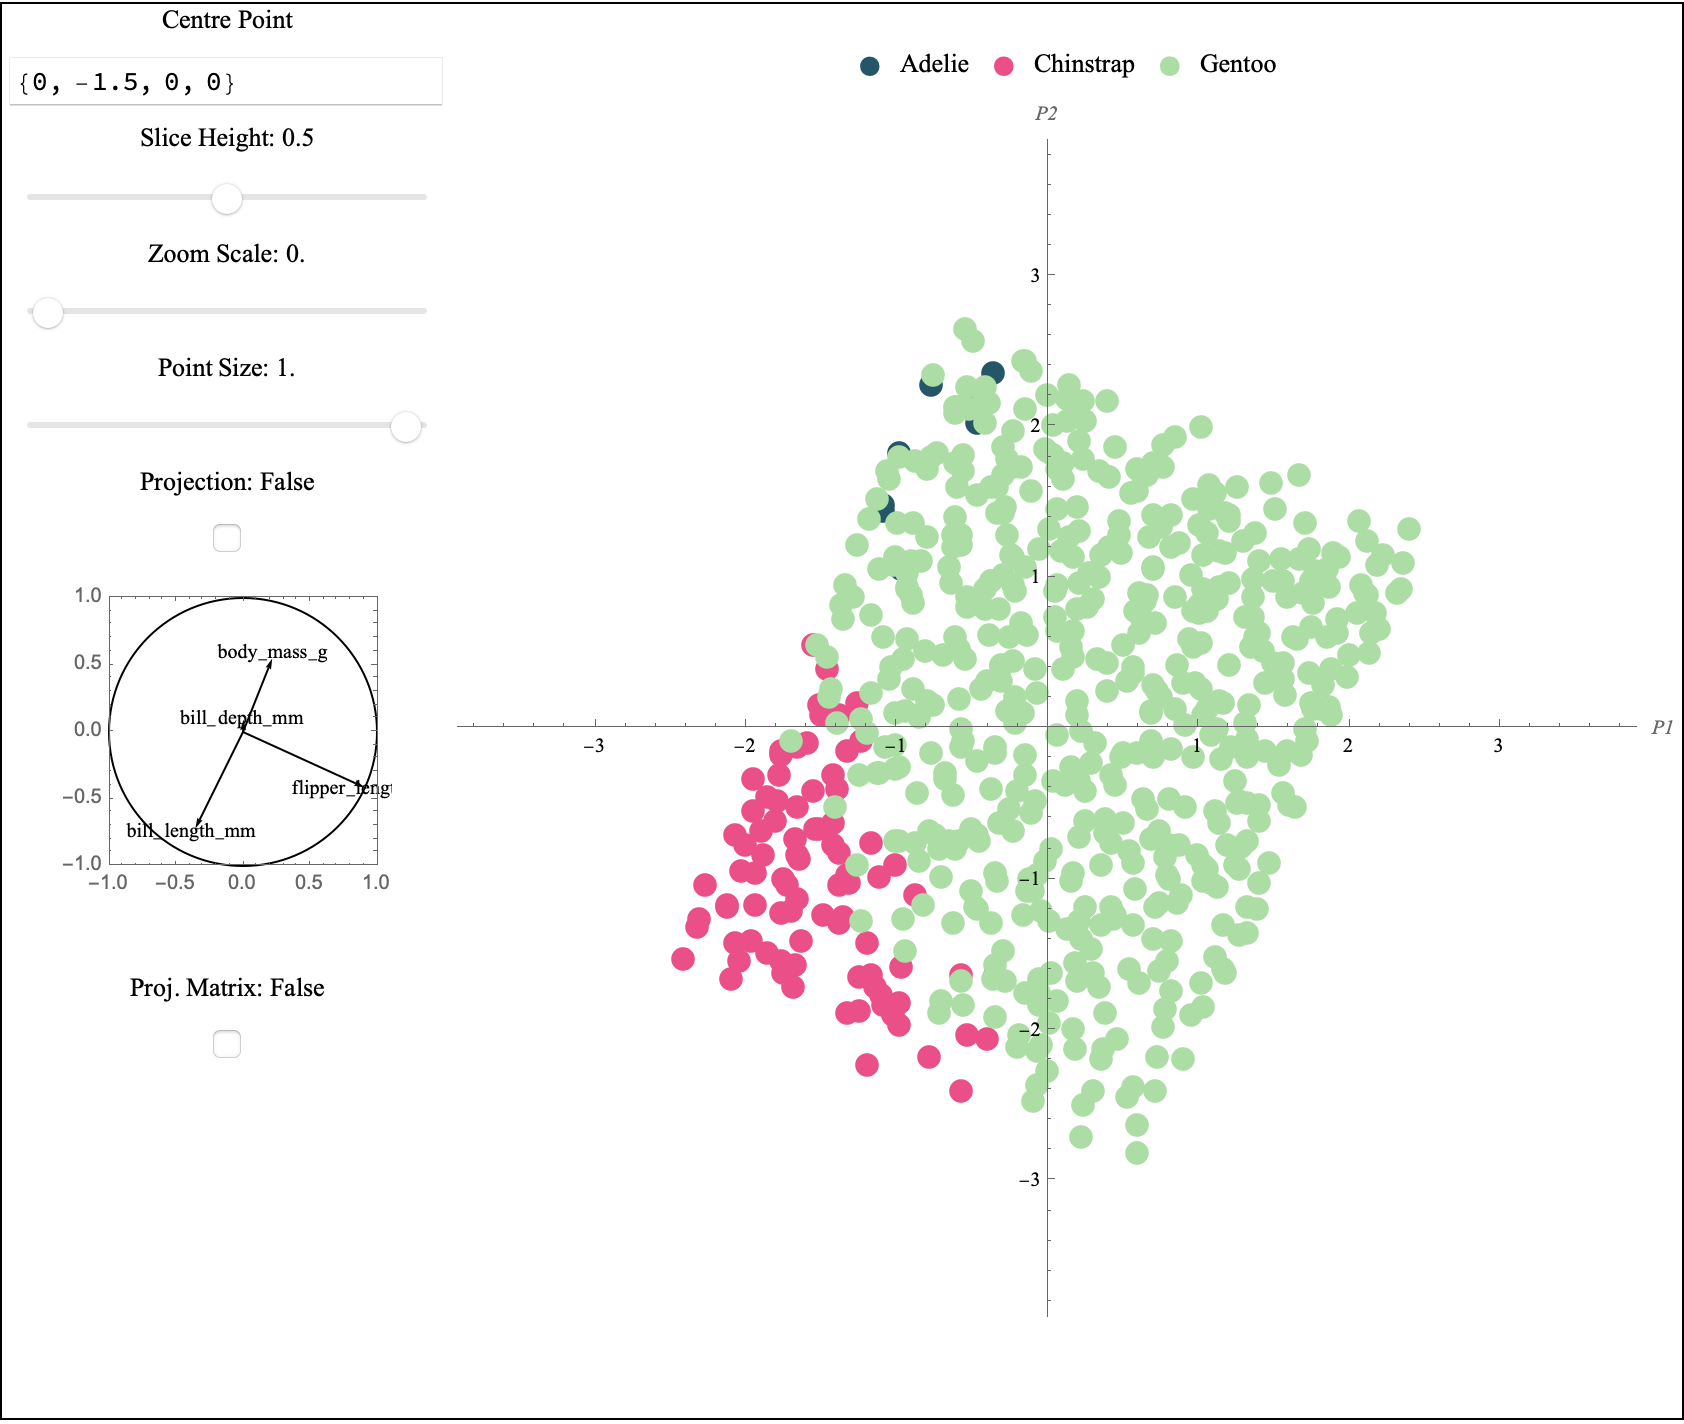
\includegraphics[width=0.32\textwidth]{figures/slice1_m_lda.png}
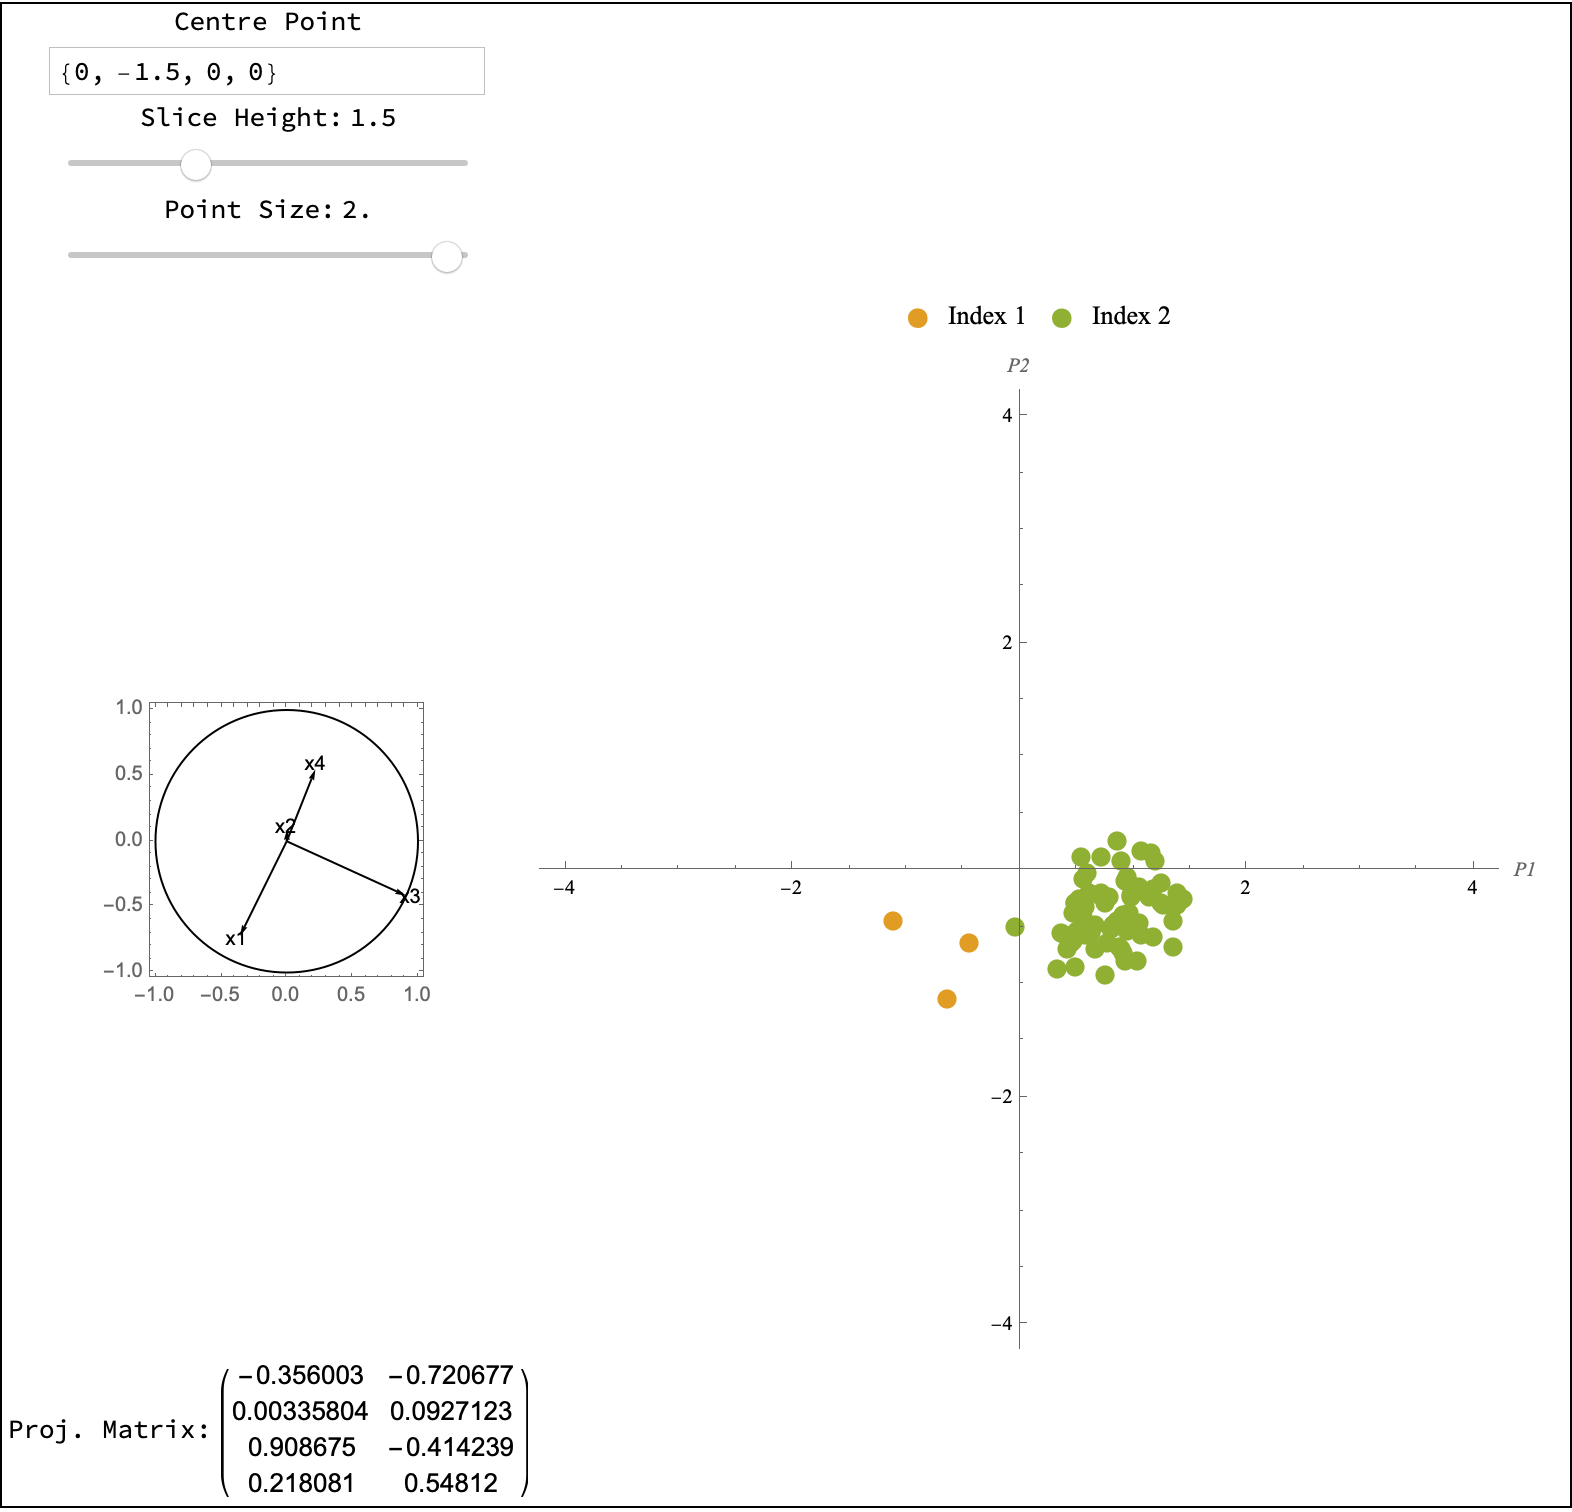
\includegraphics[width=0.32\textwidth]{figures/slice1_m_data.png}}
\caption{...}.
\label{slice1m}
\end{figure*}

Finally it is interesting to compare the slice views to the projection
of the models seen in Fig. \ref{proj1} to better understand how the
boundaries change along the \texttt{bd} direction and where the
differences in the projections come from.

\hypertarget{extension-added-in-the-r-package-tourr}{%
\section{\texorpdfstring{Extension added in the R package
\texttt{tourr}}{Extension added in the R package tourr}}\label{extension-added-in-the-r-package-tourr}}

Explain \texttt{radial\_tour}

\hypertarget{what-would-be-desirable-for-implementations-in-r}{%
\section{What would be desirable for implementations in
R?}\label{what-would-be-desirable-for-implementations-in-r}}

\hypertarget{sec:discussion}{%
\section{Discussion}\label{sec:discussion}}

\hypertarget{acknowledgements}{%
\section*{Acknowledgements}\label{acknowledgements}}
\addcontentsline{toc}{section}{Acknowledgements}

The authors gratefully acknowledge the support of the Australian
Research Council. The paper was written in \texttt{rmarkdown}
\citep{rmarkdown} using \texttt{knitr} \citep{knitr}.

\hypertarget{supplementary-material}{%
\section*{Supplementary material}\label{supplementary-material}}
\addcontentsline{toc}{section}{Supplementary material}

The source material and animated gifs for this paper are available at

\bibliographystyle{tfcad}
\bibliography{biblio.bib}





\end{document}
